\documentclass[11pt]{article}

% -----------------------------------------------------------------------------
% PaFAR working manuscript
% The source is intentionally journal-neutral and can later be migrated to an
% Elsevier, Springer, Wiley, or journal-specific class without changing content.
% -----------------------------------------------------------------------------
\usepackage[a4paper,margin=1in]{geometry}
\usepackage[T1]{fontenc}
\usepackage[utf8]{inputenc}
\usepackage{lmodern}
\usepackage{microtype}
\usepackage{setspace}
\usepackage{authblk}
\usepackage{amsmath,amssymb,amsthm,mathtools,bm}
\usepackage{bbm}
\usepackage{booktabs,threeparttable,tabularx,longtable,multirow,array,makecell}
\usepackage{graphicx}
\usepackage{tikz}
\usetikzlibrary{arrows.meta,positioning,fit,calc}
\usepackage{caption,subcaption}
\usepackage{float}
\usepackage{placeins}
\usepackage{algorithm}
\usepackage{algpseudocode}
\usepackage{enumitem}
\usepackage[dvipsnames]{xcolor}
\definecolor{pafarblue}{HTML}{2F5D7C}
\definecolor{pafarteal}{HTML}{4F7F7A}
\definecolor{pafarlight}{HTML}{EEF3F6}
\definecolor{pafargray}{HTML}{5F6B73}
\usepackage{natbib}
\usepackage{lineno}
\usepackage{url}
\usepackage[hidelinks]{hyperref}
\usepackage[nameinlink,capitalise,noabbrev]{cleveref}
\makeatletter
\@ifundefined{theHALG@line}
  {\newcommand{\theHALG@line}{\thealgorithm.\arabic{ALG@line}}}
  {\renewcommand{\theHALG@line}{\thealgorithm.\arabic{ALG@line}}}
\makeatother
\crefname{assumption}{assumption}{assumptions}
\Crefname{assumption}{Assumption}{Assumptions}
\graphicspath{{figures/}}

\onehalfspacing
\linenumbers
\setlength{\parindent}{1.5em}
\setlength{\parskip}{0.15em}
\setlist[itemize]{leftmargin=2em,itemsep=0.2em,topsep=0.3em}
\setlist[enumerate]{leftmargin=2em,itemsep=0.2em,topsep=0.3em}
\captionsetup{font=small,labelfont=bf}
\newcolumntype{L}[1]{>{\raggedright\arraybackslash}p{#1}}
\newcolumntype{Y}{>{\raggedright\arraybackslash}X}

\newtheorem{assumption}{Assumption}
\newtheorem{theorem}{Theorem}
\newtheorem{corollary}{Corollary}
\newtheorem{proposition}{Proposition}
\newtheorem{remark}{Remark}
\newtheorem{definition}{Definition}

\newcommand{\R}{\mathbb{R}}
\newcommand{\Pp}{\mathbb{P}}
\newcommand{\Ee}{\mathbb{E}}
\newcommand{\Ind}{\mathbbm{1}}
\newcommand{\calD}{\mathcal{D}}
\newcommand{\calH}{\mathcal{H}}
\newcommand{\calI}{\mathcal{I}}
\newcommand{\calT}{\mathcal{T}}
\newcommand{\calW}{\mathcal{W}}
\newcommand{\calF}{\mathcal{F}}
\newcommand{\PFA}{\operatorname{PFA}}
\newcommand{\Sens}{\operatorname{Sens}}
\newcommand{\logit}{\operatorname{logit}}
\newcommand{\expit}{\operatorname{expit}}
\newcommand{\clip}{\operatorname{clip}}
\newcommand{\argmax}{\operatorname*{arg\,max}}
\newcommand{\resultcell}{\textcolor{gray}{---}}
\newcommand{\placeholderfigure}[2]{%
  \begin{figure}[!htbp]
  \centering
  \fbox{\parbox[c][0.24\textheight][c]{0.91\linewidth}{%
    \centering\textbf{Planned real-data output}\\[0.8em]
    #1\\[0.8em]
    \textit{The PhysioNet analysis has not yet been run.}}}
  \caption{#2}
  \end{figure}}

\title{\textbf{PaFAR: Finite-Sample Patient-Level False-Alarm Control for Dynamic Clinical Early-Warning Systems}}
\author[1]{Zhuowei Gao}
\author[1]{Coauthor Name}
\author[2]{Clinical Collaborator Name}
\affil[1]{Department of Statistics, Jilin University, Changchun, China}
\affil[2]{Clinical Department and Institution, City, Country}
\date{Working manuscript, \today}

\begin{document}
\maketitle

\begin{abstract}
Dynamic clinical early-warning systems repeatedly score the same patient, so a threshold with acceptable pointwise specificity can still produce an excessive probability of at least one false alert during a monitoring episode. We propose PaFAR (Patient-level False-Alarm Risk calibration), a model-agnostic post-processing method that converts a locked score trajectory into an online alerting rule with finite-sample patient-level error control. Each non-event calibration trajectory is reduced to the maximum of a prespecified score process, and an order-statistic threshold is computed across patients. Under class-conditional exchangeability of non-event trajectories, PaFAR controls the probability that a new non-event patient receives any alert while allowing arbitrary within-patient dependence, irregular measurement, and unequal monitoring lengths. We also develop prespecified time-adaptive standardization, target-site recalibration, and a high-confidence tolerance-limit version. Primary simulations comprised 2,250 replicates across a dynamic score-process experiment and an end-to-end irregular-EHR XGBoost experiment. PaFAR-F and PaFAR-T mean PFA closely tracked the finite-sample target, whereas pointwise-alpha thresholds produced patient-level PFA of approximately 0.43--0.62 at nominal $\alpha=0.10$. Under site shift, direct source transfer yielded PFA 0.280 and 0.136 in the two experiments; recalibrating only the scalar threshold with 500 target non-events restored PFA to approximately 0.100. PaFAR-HC was more conservative and kept conditional exceedance frequencies near $\delta=0.05$ in exchangeable score-process settings. Strict patient-level reliability reduced early sensitivity, revealing a reliability--efficiency trade-off rather than a failure of calibration. The PhysioNet 2019 analysis remains a planned application.
\end{abstract}

\noindent\textbf{Keywords:} conformal calibration; clinical early warning; false alarm; irregular longitudinal data; patient-level error control; sepsis; trustworthy artificial intelligence.

\section{Introduction}

Clinical early-warning models repeatedly update a patient's risk as new electronic health record (EHR) information becomes available. In sepsis prediction, for example, a model may issue a score every hour using the current and past vital signs, laboratory measurements, missingness indicators, and demographic variables. The PhysioNet/Computing in Cardiology Challenge 2019 formalized this task through hourly predictions and a utility function that rewards timely warnings while penalizing missed events, late warnings, and false alarms \citep{reyna2019physionet,reyna2020early}. Prospective evaluations of machine-learning early-warning systems further show that deployment performance depends not only on discrimination but also on how alerts interact with clinical workflow \citep{adams2022prospective,henry2022factors}.

A central statistical mismatch remains. Most studies report AUROC, PR-AUC, calibration of individual risk scores, or sensitivity and specificity at a pointwise threshold. Clinicians, however, experience a sequence of decisions for each patient. If a non-event patient is evaluated $K$ times and the false-positive probability were $p$ independently at each time, the probability of at least one false alert would be $1-(1-p)^K$. Independence is generally unrealistic, but the calculation illustrates the more general point: pointwise specificity does not determine episode-level reliability. Repeated low-value alerts increase workload and can undermine trust, while the operational definition and measurement of alert fatigue remain heterogeneous \citep{ray2026alert}. Recent clinical-AI work has therefore considered tiered thresholds and secondary filtering to improve alert precision \citep{wu2026tiered}. The distinction between a pointwise false-positive rate and the probability of at least one false alert under repeated monitoring is not itself new; the contribution here is a patient-trajectory calibration rule whose estimand, data split, finite-sample guarantee, and deployment interpretation are aligned with dynamic clinical alerting.

Conformal prediction provides finite-sample, distribution-free guarantees for black-box prediction procedures under exchangeability \citep{vovk2005algorithmic,lei2018distribution,angelopoulos2023gentle}. Related work has developed general risk control, sequential conformal inference, and simultaneous coverage for complete trajectories \citep{bates2021distribution,angelopoulos2024conformal,xu2023sequential,zhou2024conformalized}. Conformal methods have also been applied to sepsis prediction to reduce false positives or quantify uncertainty \citep{dalal2025timeseries}. These contributions do not directly answer the operational question studied here: how should one calibrate a dynamic supervised-learning system so that a complete non-event patient episode has probability at most $\alpha$ of receiving any alert? A recent online change-point method targets a related moving-window false-positive probability \citep{martin2026sequential}, but its monitoring problem and calibration mechanism differ from the labeled patient-trajectory setting considered here.

PaFAR changes the calibration unit from an individual decision time to a complete patient trajectory. The base predictor may be XGBoost, a neural network, a regression model, or an existing clinical score. PaFAR does not refit that predictor and does not require its output to be a calibrated probability. Instead, each non-event calibration patient contributes one scalar: the largest value of a fixed, online-computable score over the prespecified monitoring episode. A split-conformal order statistic then determines the alert threshold. All serial dependence, irregular measurement frequency, and unequal episode length remain inside the patient trajectory and therefore need not be modeled for the finite-sample rank argument.

The contributions are deliberately focused.
\begin{enumerate}
    \item We define patient-level false-alarm probability as the primary reliability estimand for repeated clinical prediction and pair it with a clinically admissible early-warning sensitivity that does not reward arbitrarily premature alerts.
    \item We give a patient-trajectory calibration rule with finite-sample class-conditional control under exchangeability across non-event patients, without requiring independence across decision times within a patient or equal trajectory lengths across patients.
    \item We provide three simple extensions that preserve the same calibration logic: a prespecified time-adaptive boundary, stratum-specific or target-site recalibration, and a high-confidence nonparametric tolerance threshold.
    \item We evaluate the method in 2,250 completed primary Monte Carlo replicates spanning dynamic score processes and end-to-end irregular-EHR XGBoost pipelines. Patient-level PaFAR tracked its finite-sample target, pointwise calibration accumulated false alerts, and local scalar-threshold recalibration restored reliability under the simulated site shifts. A PhysioNet 2019 application remains planned.
\end{enumerate}

\begin{figure}[H]
\centering
\begin{tikzpicture}[
    font=\small,
    data/.style={draw=pafarblue, rounded corners=2pt, fill=pafarlight,
                 align=center, minimum height=9mm, text width=35mm,
                 inner sep=4pt, line width=0.7pt},
    process/.style={draw=pafarteal, rounded corners=2pt, fill=white,
                    align=center, minimum height=10mm, text width=39mm,
                    inner sep=4pt, line width=0.9pt},
    output/.style={draw=pafarblue, rounded corners=2pt, fill=white,
                   align=center, minimum height=10mm, text width=42mm,
                   inner sep=4pt, line width=1.0pt},
    arrow/.style={-{Latex[length=2.2mm]}, line width=0.8pt, draw=pafargray}
]
\node[data] (train) at (-4.4,2.1) {Training patients\\Fit the base learner};
\node[data] (valid) at (0,2.1) {Validation patients\\Tune the learner and fit the optional time template};
\node[data] (cal) at (4.4,2.1) {Calibration non-events\\One complete trajectory per patient};

\node[process] (locked) at (-2.2,0.35) {Freeze the causal score map\\$\mathcal H_i(t)\mapsto Z_i^{\eta}(t)$};
\node[process] (maxima) at (2.2,0.35) {Reduce each calibration\\trajectory to\\$M_i^{\eta}=\max_{t\in\mathcal I_i}Z_i^{\eta}(t)$};
\node[output] (threshold) at (2.2,-1.45) {Order-statistic calibration\\$\widehat c_{\alpha}^{\eta}=M_{(\lceil(m_0+1)(1-\alpha)\rceil)}^{\eta}$};
\node[data] (new) at (-2.2,-1.45) {New patient\\Compute scores online from current and past data only};
\node[output] (alert) at (0,-3.25) {Issue the first formal\\alert when\\$Z_{\mathrm{new}}^{\eta}(t)>\widehat c_{\alpha}^{\eta}$};

\draw[arrow] (train) -- (locked);
\draw[arrow] (valid) -- (locked);
\draw[arrow] (locked) -- (maxima);
\draw[arrow] (cal) -- (maxima);
\draw[arrow] (maxima) -- (threshold);
\draw[arrow] (locked) -- (new);
\draw[arrow] (threshold) -- (alert);
\draw[arrow] (new) -- (alert);
\end{tikzpicture}
\caption{PaFAR workflow. Training and validation determine a frozen causal score map. Each non-event calibration patient then contributes one trajectory maximum, whose order statistic defines the deployment threshold. Serial dependence and irregular observation remain inside each patient trajectory rather than being treated as independent calibration observations.}
\label{fig:pafar-workflow}
\end{figure}

The goal is not to claim that a trajectory maximum is a universally optimal alerting statistic. It is to provide a transparent reliability layer whose target, assumptions, finite-sample guarantee, implementation, and limitations can all be stated precisely. The remainder of the paper defines the estimands, presents the method and proofs, reports the simulation design and primary results, and gives the planned real-data protocol.
\section{Problem formulation}\label{sec:formulation}

\subsection{Patient trajectories and available information}

Let patients be indexed by $i=1,\ldots,n$. Patient $i$ is evaluated at ordered decision times
\[
\calT_i=\{t_{i1}<\cdots<t_{iK_i}\}.
\]
The decision grid may be regular, as in hourly ICU prediction, even when the underlying clinical variables are measured irregularly. Let $X_{ij}(s)$ denote the recorded value of variable $j$ at time $s$ when it is observed, and let $O_{ij}(s)\in\{0,1\}$ denote its observation indicator. The information available at decision time $t$ is
\begin{equation}
\calH_i(t)=\sigma\!\left\{\bm B_i,\,X_{ij}(s)O_{ij}(s),\,O_{ij}(s):s\le t,\ j=1,\ldots,p\right\},
\label{eq:history}
\end{equation}
where $\bm B_i$ contains baseline variables known before monitoring. The symbol $G_i$ is reserved below for a prespecified site or deployment stratum. Any deployed feature, score, or adaptive threshold must be measurable with respect to $\calH_i(t)$.

Let $T_i$ be the event-onset time, $H_i$ the end of the observed episode, and $D_i=\Ind(T_i\le H_i)$. Set $T_i=\infty$ when $D_i=0$. The primary monitoring set is
\begin{equation}
\calI_i=\left\{t\in\calT_i:t_{\min}\le t\le \min(H_i,H_{\max}),\ t<T_i\right\},
\label{eq:monitoring-set}
\end{equation}
where $0\le t_{\min}<H_{\max}$, and the burn-in $t_{\min}$ and administrative cap $H_{\max}$ are fixed in the analysis protocol. The cap is not required for PaFAR validity, but it defines the intended deployment episode, prevents unsupported extrapolation to extremely long stays, and makes a Bonferroni comparison well defined.

For theoretical purposes, write $\mathcal O_i$ for the complete labeled trajectory of patient $i$, including its baseline variables, monitoring times, observation pattern, observed history, episode end, and event label. The map from $\mathcal O_i$ to the patient-level calibration score will be fixed before the calibration sample is examined.

\subsection{Locked dynamic risk score and causal smoothing}

A base learner is fitted on a patient-level training set and tuned on a separate validation set. After tuning, the entire prediction pipeline is frozen. At each decision time,
\begin{equation}
R_i(t)=\widehat f\{\calH_i(t)\}\in[0,1]
\label{eq:base-risk}
\end{equation}
is a score for event onset during a prespecified future horizon $h$. PaFAR does not require $R_i(t)$ to equal the true conditional event probability; calibration is applied to the alert policy rather than to the probability scale. The range $[0,1]$ matches the planned logistic learner. A real-valued clinical score can instead be used with a fixed nondecreasing transformation defined on its range; the validity argument requires only that the same frozen score map be used for calibration and deployment.

To reduce isolated numerical spikes, the primary implementation uses a causal moving average over the most recent $L$ decision scores. For $r=1,\ldots,K_i$, let $L_{ir}=\min(L,r)$ and define
\begin{equation}
\widetilde R_i(t_{ir})=
\frac{1}{L_{ir}}\sum_{\ell=0}^{L_{ir}-1}R_i(t_{i,r-\ell}).
\label{eq:smooth-score}
\end{equation}
The primary analysis fixes $L=3$ before final calibration; $L=1$ is a sensitivity analysis. Equation~\eqref{eq:smooth-score} remains causal on an irregular decision grid because it uses only current and previous decision times.

\subsection{Predictable score standardization and trajectory maximum}

Let $V_i(t)$ be a vector of variables known at time $t$, such as elapsed monitoring time or recent measurement count. Let $\phi:[0,1]\rightarrow\R$ be a fixed nondecreasing transformation. The default is the clipped logit
\begin{equation}
\phi(r)=\log\left\{
\frac{\clip(r,\varepsilon,1-\varepsilon)}
{1-\clip(r,\varepsilon,1-\varepsilon)}
\right\},
\qquad
\clip(r,a,b)=\min\{\max(r,a),b\},
\label{eq:score-transform}
\end{equation}
with $\varepsilon=10^{-6}$. For a template $\eta=(a_\eta,b_\eta)$ fixed before calibration, define
\begin{equation}
Z_i^{\eta}(t)=
\frac{\phi\{\widetilde R_i(t)\}-a_\eta\{V_i(t)\}}
{b_\eta\{V_i(t)\}},
\qquad b_\eta(v)\ge b_{\min}>0.
\label{eq:standardized-score}
\end{equation}
The fixed-boundary method has $a_\eta\equiv0$ and $b_\eta\equiv1$. A prespecified time-adaptive template is given in \Cref{subsec:adaptive}.

The scalar calibration score for patient $i$ is
\begin{equation}
M_i^{\eta}=\max_{t\in\calI_i}Z_i^{\eta}(t),
\label{eq:trajectory-score}
\end{equation}
with $M_i^{\eta}=-\infty$ when $\calI_i$ is empty. Serial dependence, irregular observation, and monitoring length affect the distribution of $M_i^{\eta}$ but do not need to be modeled separately in the validity proof.

\subsection{Alert rule and estimands}

For a threshold $c$, the first formal alert time is
\begin{equation}
\tau_i(c)=\inf\{t\in\calI_i:Z_i^{\eta}(t)>c\},
\qquad \inf(\varnothing)=\infty.
\label{eq:first-alert}
\end{equation}
Because the crossing inequality is strict,
\[
\{\tau_i(c)<\infty\}=\{M_i^{\eta}>c\}.
\]
The patient-level reliability analysis uses only this first crossing. For the secondary burden analysis, let the first alert episode start at $e_{i1}=\tau_i(c)$. A subsequent episode starts at the earliest new upcrossing that occurs at least six hours after the preceding episode start and only after the score has returned to or below the threshold at an intervening decision time. This rule is applied recursively and fixes the alert-episode count used below. The auxiliary PhysioNet utility calculation is defined separately in \Cref{sec:realdata}; it is not used to define, tune, or calibrate the first-alert rule.

\begin{definition}[Patient-level false-alarm probability]
For a non-event patient, define
\begin{equation}
\PFA_{\mathrm{patient}}(c)
=\Pp\{\tau_i(c)<\infty\mid D_i=0\}
=\Pp\{M_i^{\eta}>c\mid D_i=0\}.
\label{eq:pfa}
\end{equation}
The reliability target is $\PFA_{\mathrm{patient}}(c)\le\alpha$.
\end{definition}

For event patients, an alert should be early enough to permit action but not so early that it is clinically unrelated to the impending event. Let $W_{\max}>0$ be the largest admissible lead time and let $\ell\in[0,W_{\max})$ be the required minimum lead. Define the evaluable warning set
\begin{equation}
\calW_{i,\ell}=\calI_i\cap[T_i-W_{\max},T_i-\ell],
\label{eq:evaluable-window}
\end{equation}
where the monitoring set $\calI_i$ already excludes $t\ge T_i$. The lead-specific sensitivity is
\begin{equation}
\Sens_{\ell}(c)=
\Pp\{T_i-W_{\max}\le\tau_i(c)\le T_i-\ell
\mid D_i=1,\calW_{i,\ell}\ne\varnothing\}.
\label{eq:lead-sensitivity}
\end{equation}
The primary six-hour prediction analysis sets $W_{\max}=h=6$ hours. It reports $\Sens_3$, which requires at least three hours of lead time, and $\Sens_0$, which counts any first alert during the six-hour pre-onset window. Among event patients evaluable at $\ell=0$, the premature-alert probability is
\begin{equation}
\Pp\{\tau_i(c)<T_i-W_{\max}\mid D_i=1,
\calW_{i,0}\ne\varnothing\}.
\label{eq:premature}
\end{equation}
The lead-specific positive predictive value is
\begin{equation}
\operatorname{PPV}_{\ell}(c)=
\Pp\{D_i=1,\ T_i-W_{\max}\le\tau_i(c)\le T_i-\ell
\mid \tau_i(c)<\infty\}.
\label{eq:lead-ppv}
\end{equation}
Thus an event patient whose first alert occurs before the six-hour prediction window is counted as premature rather than as a valid detection. In the main tables, the unqualified ``PPV'' denotes $\operatorname{PPV}_3$, aligned with the primary three-hour-lead sensitivity; $\operatorname{PPV}_0$ is reported as a supplementary sensitivity measure. The estimands deliberately have different denominators: patient PFA uses all non-event patients in the analysis cohort; $\Sens_{\ell}$ uses only event patients with $\calW_{i,\ell}\ne\varnothing$; and $\operatorname{PPV}_{\ell}$ conditions on every patient who receives a formal first alert. Consequently, an event patient with a premature alert, or an event patient who is not evaluable for $\Sens_{\ell}$, remains in the PPV and alert-burden population but does not contribute a valid-detection numerator.

Secondary summaries include median lead time among detections counted by $\Sens_0$, alert episodes per 100 patient-days, the cumulative probability of a first false alert by elapsed time, weighted trapezoidal PR-AUC, AUROC, and the official PhysioNet utility. Threshold-free metrics describe the score generator; equations~\eqref{eq:pfa}--\eqref{eq:lead-ppv} describe the deployed alert policy.

\subsection{Patient-level data separation}

Patients are divided into mutually disjoint sets
\[
\calD_{\mathrm{tr}},\qquad
\calD_{\mathrm{val}},\qquad
\calD_{\mathrm{cal}},\qquad
\calD_{\mathrm{te}}.
\]
The training set fits the base model. The validation set selects learner hyperparameters and fits any adaptive template. The calibration set is used once to compute the final patient-level threshold. The test set is used only for final evaluation. No time points from the same patient may appear in different sets. Event patients in the calibration set are not used to estimate the non-event false-alarm threshold.
\section{PaFAR methodology}\label{sec:method}

\subsection{Fixed-boundary patient-level calibration}

Let
\[
\calD_{\mathrm{cal},0}=\{i\in\calD_{\mathrm{cal}}:D_i=0\}
\]
contain $m_0$ non-event calibration patients. For a frozen template $\eta$, compute the patient scores in \eqref{eq:trajectory-score} and order them as
\[
M_{(1)}^{\eta}\le\cdots\le M_{(m_0)}^{\eta}.
\]
Define the augmented order statistic $M_{(m_0+1)}^{\eta}=+\infty$. For a target $\alpha\in(0,1)$, set
\begin{equation}
k_{\alpha}(m_0)=\left\lceil(m_0+1)(1-\alpha)\right\rceil,
\qquad
\widehat c_{\alpha}^{\eta}=M_{(k_{\alpha}(m_0))}^{\eta}.
\label{eq:conformal-threshold}
\end{equation}
The deployed rule alerts when
\begin{equation}
Z_{\mathrm{new}}^{\eta}(t)>\widehat c_{\alpha}^{\eta}.
\label{eq:alert-rule}
\end{equation}
The strict inequality handles tied scores conservatively. A non-augmented order-statistic threshold is available exactly when
\begin{equation}
m_0\ge \left\lceil\frac{1}{\alpha}\right\rceil-1;
\label{eq:min-cal-marginal}
\end{equation}
otherwise $k_{\alpha}(m_0)=m_0+1$ and the certified rule never alerts. This behavior is preferable to reporting an unsupported empirical threshold when the calibration sample is too small.

\subsection{Prespecified time-adaptive PaFAR}\label{subsec:adaptive}

A single raw-score threshold can be inefficient when non-event scores drift with elapsed time. PaFAR therefore permits a predictable location-scale template estimated from validation non-events and frozen before final calibration. This template changes efficiency but not the rank argument.

Let $U_i(t)=\phi\{\widetilde R_i(t)\}$. To avoid boundary ambiguities when $t_{\min}$ changes in a sensitivity analysis, first form
\[
\mathcal C=\{t_{\min},H_{\max}\}\cup
\bigl(\{12,24,48,72\}\cap(t_{\min},H_{\max})\bigr).
\]
Write the sorted distinct elements of $\mathcal C$ as
\[
c_0=t_{\min}<c_1<\cdots<c_B=H_{\max}.
\]
Define
\begin{equation}
b_1=[c_0,c_1],\qquad b_r=(c_{r-1},c_r],\quad r=2,\ldots,B,
\label{eq:time-bins}
\end{equation}
and write $\mathcal B_0=\{b_1,\ldots,b_B\}$ for this initial unmerged partition. Thus the primary setting $t_{\min}=6$ and $H_{\max}>72$ gives $[6,12],(12,24],(24,48],(48,72],(72,H_{\max}]$, while every alternative $t_{\min}$ remains fully covered. Data-empty intervals are retained initially so that the final template covers the entire monitoring range. For a candidate bin $b$, let
\[
n_{ib}=\sum_{t\in\calI_i}\Ind(t\in b),
\qquad
N_b=\sum_{i\in\calD_{\mathrm{val},0}}\Ind(n_{ib}>0),
\]
where $\calD_{\mathrm{val},0}$ denotes validation non-events.

Bin merging is deterministic and is performed before any location or scale is estimated. At each iteration, identify the latest remaining bin with $N_b<50$. If it is not the first bin, merge it with its immediate predecessor; if it is the first bin and another bin remains, merge it with its immediate successor. Recompute all counts and repeat until every remaining bin has at least 50 contributing patients or only one bin remains. The complete partition and all merges are fixed using validation non-events before calibration data are accessed. If the single remaining bin has $N_b=0$, set $\widehat a_b=0$ and $\widehat b_b=1$, so PaFAR-T deterministically reduces to PaFAR-F; otherwise the estimates below are used even if the final single bin has fewer than 50 contributors. Let $\widehat{\mathcal B}_{\mathrm{T}}$ denote the final validation-derived partition after this merging procedure.

For each resulting bin with $N_b>0$, recompute $n_{ib}$ and $N_b$ and define the patient-equalized weighted empirical distribution
\begin{equation}
\widehat F_b(u)=\frac{1}{N_b}
\sum_{i\in\calD_{\mathrm{val},0}:n_{ib}>0}
\frac{1}{n_{ib}}\sum_{t\in\calI_i\cap b}\Ind\{U_i(t)\le u\}.
\label{eq:weighted-cdf}
\end{equation}
The location estimate is the weighted median
\[
\widehat a_b=\inf\{u:\widehat F_b(u)\ge1/2\}.
\]
Using the same patient-equalized weights, let
\begin{equation}
\widehat d_b=
\inf\left\{d\ge0:
\frac{1}{N_b}
\sum_{i:n_{ib}>0}\frac{1}{n_{ib}}
\sum_{t\in\calI_i\cap b}
\Ind\{|U_i(t)-\widehat a_b|\le d\}\ge\frac12
\right\},
\label{eq:weighted-mad}
\end{equation}
and set
\begin{equation}
\widehat b_b=\max\{1.4826\widehat d_b,\ b_{\min}\},
\qquad b_{\min}=0.10.
\label{eq:scale-floor}
\end{equation}
The factor 1.4826 makes the median absolute deviation consistent for a Gaussian scale; neither validity nor implementation assumes Gaussian scores. Each contributing patient receives total weight one within a bin, so a long trajectory does not dominate template estimation.

For $t\in b$, the time-adaptive score is
\begin{equation}
Z_i^{\mathrm{T}}(t)=
\frac{U_i(t)-\widehat a_b}{\widehat b_b}.
\label{eq:time-adaptive-score}
\end{equation}
The corresponding online boundary on the transformed risk scale is
\begin{equation}
U_{\mathrm{new}}(t)>
\widehat a_b+\widehat c_{\alpha}^{\mathrm{T}}\widehat b_b.
\label{eq:adaptive-boundary}
\end{equation}
We call the fixed method PaFAR-F and the time-adaptive method PaFAR-T. Both are prespecified and reported; no search over calibration-set performance is permitted. Observation-intensity variables may be incorporated in a secondary analysis, but they are not needed for the primary method or simulation.

\subsection{Stratum-specific and target-site recalibration}

Let $G_i\in\{1,\ldots,G\}$ be a stratum known before any alert can occur, such as hospital or ICU type. If stratum $g$ contains $m_{0g}$ non-event calibration patients, order their trajectory scores, set $M_{g,(m_{0g}+1)}^{\eta}=+\infty$, and define
\begin{equation}
\widehat c_{\alpha,g}^{\eta}
=M_{g,(k_{\alpha}(m_{0g}))}^{\eta}.
\label{eq:stratum-threshold}
\end{equation}
This yields a separate patient-level threshold within each prespecified stratum. Final length of stay is not an admissible stratum because it is unknown at the time of alerting.

For external deployment, the base learner and adaptive template may be developed at source site A, while only the scalar threshold is recalibrated using non-event trajectories from target site B. The target threshold then controls target-site false alerts if the target calibration non-events are exchangeable with future target non-events. Applying the source threshold unchanged is retained as a transfer baseline but has no distribution-free guarantee under site shift.

\subsection{Optional high-confidence PaFAR}

The threshold in \eqref{eq:conformal-threshold} gives a marginal guarantee jointly over a random calibration set and a new patient. A realized calibration set may nevertheless produce a conditional deployment risk above $\alpha$. To obtain a high-probability statement about the realized rule, choose $\delta\in(0,1)$ and define
\begin{equation}
k_{\alpha,\delta}^{\mathrm{HC}}(m_0)
=\min\left\{k\in\{1,\ldots,m_0+1\}:
\sum_{j=k}^{m_0}\binom{m_0}{j}(1-\alpha)^j\alpha^{m_0-j}
\le\delta\right\},
\label{eq:hc-index}
\end{equation}
where the sum is zero for $k=m_0+1$. The high-confidence threshold is
\begin{equation}
\widehat c_{\alpha,\delta}^{\mathrm{HC},\eta}
=M_{(k_{\alpha,\delta}^{\mathrm{HC}}(m_0))}^{\eta}.
\label{eq:hc-threshold}
\end{equation}
This is a one-sided distribution-free tolerance limit \citep{wilks1941determination}. A non-augmented high-confidence threshold index exists if and only if
\begin{equation}
(1-\alpha)^{m_0}\le\delta,
\qquad\text{equivalently}\qquad
m_0\ge\left\lceil\frac{\log\delta}{\log(1-\alpha)}\right\rceil.
\label{eq:hc-min-sample}
\end{equation}
For example, $\delta=0.05$ requires at least 59 non-event calibration patients when $\alpha=0.05$ and at least 29 when $\alpha=0.10$. Larger samples are usually needed for a practically useful threshold because the qualifying order statistic can be very high.

\subsection{Implementation algorithms}

\begin{algorithm}[H]
\caption{PaFAR fitting and calibration}
\label{alg:calibration}
\begin{algorithmic}[1]
\Require Patient-level training, validation, and calibration sets; target $\alpha$; optional $\delta$.
\State Train each candidate base risk model using the training patients only.
\State Select learner hyperparameters and the boosting round using the validation patients only, including validation-based early stopping.
\State Freeze the selected base risk model; do not refit it on the union of the training and validation patients.
\State Fix all feature definitions, the causal smoother, the monitoring rule, and the score transformation.
\State For PaFAR-T, estimate the time-bin locations and scales from validation non-events using \eqref{eq:weighted-cdf}--\eqref{eq:scale-floor}; then freeze the template.
\State Retain the $m_0$ non-event calibration patients and compute one trajectory maximum $M_i^{\eta}$ per patient.
\State Sort the $m_0$ maxima.
\If{marginal PaFAR is used}
    \State Set $\widehat c=\widehat c_{\alpha}^{\eta}$ from \eqref{eq:conformal-threshold}.
\Else
    \State Set $\widehat c=\widehat c_{\alpha,\delta}^{\mathrm{HC},\eta}$ from \eqref{eq:hc-threshold}.
\EndIf
\State \Return the locked prediction pipeline, optional adaptive template, and scalar threshold $\widehat c$.
\end{algorithmic}
\end{algorithm}

\begin{algorithm}[H]
\caption{Online deployment for a new patient}
\label{alg:online}
\begin{algorithmic}[1]
\Require Locked pipeline and threshold $\widehat c$.
\For{each eligible decision time $t$}
    \State Construct features from $\calH_{\mathrm{new}}(t)$ only.
    \State Compute $R_{\mathrm{new}}(t)$, $\widetilde R_{\mathrm{new}}(t)$, and $Z_{\mathrm{new}}^{\eta}(t)$.
    \If{$Z_{\mathrm{new}}^{\eta}(t)>\widehat c$ and no previous formal alert has occurred}
        \State Issue the formal alert and set $\tau_{\mathrm{new}}=t$.
    \EndIf
\EndFor
\end{algorithmic}
\end{algorithm}

Let $J_i=|\calI_i|$. Constructing the calibration maxima requires $O\!\left(\sum_{i\in\calD_{\mathrm{cal},0}}J_i\right)$ score scans, after which sorting requires $O(m_0\log m_0)$ time and storing the maxima requires $O(m_0)$ memory. If locked score trajectories have already been generated, the additional calibration overhead is therefore $O(m_0\log m_0)$. Online PaFAR adds only a fixed transformation and one threshold comparison to the base prediction pipeline.

\section{Finite-sample guarantees}\label{sec:theory}

Let $\calF_{\mathrm{fit}}$ be the sigma-field generated by the training and validation data, fitted learner, feature definitions, smoothing rule, monitoring rule, adaptive template, and any prespecified stratum definitions. All results below are conditional on $\calF_{\mathrm{fit}}$.

\begin{assumption}[Patient-level class-conditional exchangeability]\label{ass:exchangeability}
Conditional on $\calF_{\mathrm{fit}}$, the observed number $m_0$ of calibration non-events, and $D_{\mathrm{new}}=0$, the $m_0$ calibration non-event trajectories and the new non-event trajectory are exchangeable. Exchangeability is required across patients, not across decision times within a patient.
\end{assumption}

\begin{assumption}[Frozen and online-computable score map]\label{ass:frozen}
The map $\mathcal O_i\mapsto M_i^{\eta}$ is the same for calibration and deployment patients and is fixed before calibration scores are examined. At every decision time, all features, smoothing operations, and adaptive variables use only current and past information. No patient contributes data to more than one analysis split.
\end{assumption}

\begin{assumption}[Common monitoring episode]\label{ass:stable-episode}
The eligible set $\calI_i$ is generated by the same prespecified rule for calibration and deployment patients. In the retrospective analysis, the hypothetical PaFAR alert does not change subsequent measurement, treatment, discharge, event labeling, or episode length.
\end{assumption}

\begin{theorem}[Finite-sample patient-level false-alarm control]\label{thm:marginal}
Under \Cref{ass:exchangeability,ass:frozen,ass:stable-episode}, let $\widehat c_{\alpha}^{\eta}$ be defined by \eqref{eq:conformal-threshold}. Then
\begin{align}
&\Pp\left\{\exists t\in\calI_{\mathrm{new}}:
Z_{\mathrm{new}}^{\eta}(t)>\widehat c_{\alpha}^{\eta}
\ \middle|\ D_{\mathrm{new}}=0,\calF_{\mathrm{fit}},m_0\right\}
\nonumber\\
&\hspace{4em}\le
\frac{m_0+1-k_{\alpha}(m_0)}{m_0+1}
\le\alpha.
\label{eq:theorem-marginal}
\end{align}
The result permits arbitrary within-patient temporal dependence, irregular observation patterns, and unequal monitoring lengths across patients.
\end{theorem}

\begin{corollary}[Validity of validation-fitted adaptive templates]\label{cor:adaptive}
Let $\widehat\eta$ be any template measurable with respect to $\calF_{\mathrm{fit}}$, including the time-adaptive template in \eqref{eq:time-adaptive-score}. If the frozen template is applied identically to calibration and deployment patients, \Cref{thm:marginal} holds with $\eta=\widehat\eta$.
\end{corollary}

\begin{remark}[Scope of the trajectory-level guarantee]\label{rem:marginal-scope}
The guarantee in \Cref{thm:marginal} is marginal over the prespecified distribution of complete non-event monitoring trajectories, including their monitoring lengths, observation patterns, and measurement intensities. It does not imply false-alarm control conditional on a duration group, observation-intensity group, or other subgroup unless that subgroup is prespecified and receives its own independently calibrated threshold as in \Cref{thm:stratum}. In particular, a descriptive false-alert rate among the longest-stay patients may exceed $\alpha$ even when the overall patient-level guarantee holds.
\end{remark}

\begin{theorem}[Stratum-specific control, including target-site recalibration]\label{thm:stratum}
Suppose $G_i=g$ is known before alerting and the calibration and deployment non-event trajectories are exchangeable conditional on $G_i=g$. Under \Cref{ass:frozen,ass:stable-episode}, the threshold in \eqref{eq:stratum-threshold} satisfies
\begin{equation}
\Pp\{\tau_{\mathrm{new}}(\widehat c_{\alpha,g}^{\eta})<\infty
\mid D_{\mathrm{new}}=0,G_{\mathrm{new}}=g,
\calF_{\mathrm{fit}},m_{0g}\}\le\alpha.
\label{eq:stratum-control}
\end{equation}
If every prespecified stratum is calibrated at level $\alpha$, the unconditional non-event false-alarm probability, averaged over the deployment stratum distribution, is also at most $\alpha$. In particular, when a source-fitted score map is frozen and $G_i$ indexes the target site, a threshold recalibrated from target-site non-events has the same guarantee for future exchangeable target-site non-events.
\end{theorem}

\begin{assumption}[Sampling condition for high-confidence control]\label{ass:hc}
Conditional on $\calF_{\mathrm{fit}}$, $m_0$, and the non-event class, the calibration scores are independent and identically distributed with
\[
F_0(x)=\Pp\{M_i^{\eta}\le x\mid D_i=0,\calF_{\mathrm{fit}}\},
\]
and the future non-event score is an independent draw from the same distribution. Continuity of $F_0$ is not required.
\end{assumption}

\begin{theorem}[High-confidence deployment-conditional control]\label{thm:hc}
Under \Cref{ass:frozen,ass:stable-episode,ass:hc}, let $\widehat c_{\alpha,\delta}^{\mathrm{HC},\eta}$ be defined by \eqref{eq:hc-threshold}. Then
\begin{equation}
\Pp_{\calD_{\mathrm{cal},0}}\!\left[
\Pp\left\{M_{\mathrm{new}}^{\eta}>
\widehat c_{\alpha,\delta}^{\mathrm{HC},\eta}
\mid\calD_{\mathrm{cal},0},D_{\mathrm{new}}=0,
\calF_{\mathrm{fit}}\right\}>\alpha
\right]\le\delta.
\label{eq:hc-guarantee}
\end{equation}
The outer probability in \eqref{eq:hc-guarantee} is conditional on $\calF_{\mathrm{fit}}$ and the realized count $m_0$. Hence, with probability at least $1-\delta$ over the calibration sample, the conditional patient-level false-alarm probability of the realized deployed rule is at most $\alpha$.
\end{theorem}

\begin{remark}[Marginal and conditional statements]
\Cref{thm:marginal} controls the joint probability over a random calibration sample and a new patient. It does not imply that every realized marginal-PaFAR threshold has conditional risk below $\alpha$. \Cref{thm:hc} supplies that stronger high-probability statement under the additional i.i.d. sampling condition, at the cost of a more conservative threshold.
\end{remark}

\begin{remark}[Distribution shift and intervention feedback]
A source-site threshold transferred unchanged to a non-exchangeable target population is not protected by \Cref{thm:marginal}. Target-site recalibration restores the rank guarantee only when target calibration patients represent future target deployment patients. Likewise, a prospective alert that changes subsequent care can alter the trajectory distribution; prospective monitoring and periodic recalibration are then required.
\end{remark}
\section{Base learner and irregular-EHR features}\label{sec:learner}

\subsection{Hourly prediction labels}

For a prediction horizon $h=6$ hours, model fitting uses the eligible decision times $t\in\calI_i$, and the binary training label at a pre-onset decision time is
\begin{equation}
Y_i(t)=\Ind\{D_i=1,\ 0<T_i-t\le h\},
\qquad t<T_i.
\label{eq:hour-label}
\end{equation}
Hours at or after onset are excluded from model fitting and from the primary discrimination and first-alert evaluations. This prevents a model from appearing accurate merely because it recognizes an already established event. The auxiliary PhysioNet utility analysis in \Cref{sec:realdata} is the only evaluation that retains post-onset hours, because the official scoring rule requires the complete hourly prediction vector.

Long-stay patients contribute more hourly records. We therefore begin with patient-equal base weights and then balance the two hourly classes in aggregate. All patients used for learner fitting must have $K_i^{\mathrm{fit}}>0$. Let $n_{\mathrm{tr}}^{+}$ be the number of training patients with at least one eligible fitting time and define the patient-weighted positive fraction
\begin{equation}
\widehat\pi_Y=
\frac{1}{n_{\mathrm{tr}}^{+}}
\sum_{i\in\calD_{\mathrm{tr}}:K_i^{\mathrm{fit}}>0}
\frac{1}{K_i^{\mathrm{fit}}}
\sum_{t}Y_i(t).
\label{eq:weighted-prevalence}
\end{equation}
The unnormalized fitting weight is
\begin{equation}
w_i(t)=\frac{1}{K_i^{\mathrm{fit}}}
\left\{
\frac{Y_i(t)}{2\widehat\pi_Y}
+\frac{1-Y_i(t)}{2(1-\widehat\pi_Y)}
\right\},
\label{eq:patient-weight}
\end{equation}
followed by a common rescaling so that the mean training weight is one. The implementation must verify $0<\widehat\pi_Y<1$ before these weights are formed. For learner tuning and early stopping, each eligible validation hour instead receives weight $1/K_i^{\mathrm{fit}}$, followed by a common rescaling; no additional class balancing is applied to the validation metric. The reference implementation uses the native \texttt{xgboost.train} interface, places the validation \texttt{DMatrix} last (or uses it as the only evaluation set), and sets XGBoost's weighted \texttt{aucpr} as the final evaluation metric. This raw-score metric selects the learner configuration and boosting round. All subsequent predictions explicitly use \texttt{iteration\_range} $=(0,\texttt{best\_iteration}+1)$; trees grown after the best iteration are not used. The three-score smoother is applied only after selection, which keeps learner fitting separate from alert-policy post-processing. For threshold-free reporting on the smoothed score $\widetilde R_i(t)$, weighted PR-AUC is computed by \texttt{sklearn.metrics.precision\_recall\_curve} with the patient-equal test weights followed by \texttt{sklearn.metrics.auc(recall, precision)}; weighted AUROC uses \texttt{roc\_auc\_score} with the same weights. The reporting PR-AUC is therefore explicitly distinguished from XGBoost's raw-score early-stopping \texttt{aucpr}, and neither quantity is called average precision. Raw-score discrimination metrics are a sensitivity analysis. If the training or validation labels contain only one class, the replicate is recorded as a learner-fitting failure and is not silently regenerated or assigned an artificial metric value. The exact implementation and software versions are recorded. An unweighted-hour analysis is also reported as a sensitivity analysis.

\subsection{Causal feature construction}

At each decision time, the primary feature set contains the following for each longitudinal physiological variable. This means the 34 vital-sign and laboratory variables in the PhysioNet analysis and the 12 generated biomarkers in Experiment II; baseline and administrative variables are entered separately and are not subjected to rolling summaries:
\begin{itemize}
    \item last observed value, an indicator that the variable has never been observed, and time since the last observation;
    \item mean, minimum, maximum, and sample standard deviation over the previous 6, 12, and 24 hours;
    \item net change and ordinary least-squares slope over each window when at least two distinct measurement times are present;
    \item number of measurements in each window and a current-hour observation indicator.
\end{itemize}
For a window of width $w$, ``previous $w$ hours'' means observations with timestamps $s\in(t-w,t]$; on the hourly grid this contains at most the current hour and the preceding $w-1$ hours. Net change is the latest minus the earliest observed value in that window, and the slope uses elapsed hours as the time coordinate. The sample standard deviation, net change, and slope are undefined when their required measurement counts are not met. Baseline age, sex, hospital source, available unit indicators, elapsed ICU time, and hospital-admission offset are then added as separate predictors. Age, sex, unit indicators, hospital source, and hospital-admission offset are not expanded into rolling-window features; elapsed ICU time is the current causal time coordinate. An undefined numerical summary is replaced by the median of its finite values in the training set and accompanied by a missingness indicator; if no finite training value exists, the replacement is zero. No value is backfilled from the future. Observation counts and time since last measurement are retained because the measurement process itself may contain predictive information \citep{che2018recurrent}.

\subsection{Primary learner and fixed tuning protocol}

The primary learner is XGBoost with a logistic objective \citep{chen2016xgboost}. For the real-data analysis, the validation grid is
\begin{align*}
\texttt{max\_depth}&\in\{2,3,4\},&
\texttt{eta}&\in\{0.03,0.05,0.10\},\\
\texttt{min\_child\_weight}&\in\{1,5\},&
\texttt{subsample}&=0.80,\\
\texttt{colsample\_bytree}&=0.80.&&
\end{align*}
The number of boosting rounds is at most 800 with early stopping after 40 rounds without improvement. The selected model maximizes the patient-weighted validation \texttt{aucpr} value; ties are resolved by smaller depth, then smaller learning rate, then larger \texttt{min\_child\_weight}, and finally fewer boosting rounds. The recorded boosting-round count is $\texttt{best\_iteration}+1$, because \texttt{best\_iteration} is zero based. Threshold choice is not part of learner tuning.

To keep the repeated end-to-end simulation computationally feasible and to isolate the behavior of the calibration layer, Experiment II does not rerun the full hyperparameter grid in every replicate. It fixes \texttt{max\_depth}$=3$, \texttt{eta}$=0.05$, \texttt{min\_child\_weight}$=5$, \texttt{subsample}$=0.80$, and \texttt{colsample\_bytree}$=0.80$; only the number of boosting rounds is selected by patient-weighted validation \texttt{aucpr}, with at most 400 rounds and early stopping after 25 non-improving rounds. This separation keeps discrimination learning distinct from patient-level alert calibration and makes the simulation directly reproducible.

The three-score causal average in \eqref{eq:smooth-score} is fixed as the primary score. Raw scores are reported in a sensitivity analysis. A regularized logistic regression using the same features may be included as a secondary score generator, but it is not required for the central simulation or theoretical claims.

\section{Simulation study}\label{sec:simulation}

\subsection{Design principles}

The simulation has two complementary components. Experiment I directly generates score trajectories and changes one mechanism at a time for precise evaluation of finite-sample calibration. Experiment II generates irregular longitudinal biomarkers, constructs causal features, refits XGBoost, and then applies the same calibration procedures in a small number of deliberately bundled end-to-end stress tests. The design avoids a large factorial crossing of every parameter. This keeps the computation feasible while separating mechanism checks from realistic pipeline checks.

The common primary values are $\alpha=0.10$, $\delta=0.05$, event prevalence $\pi=0.10$, burn-in $t_{\min}=6$, maximum monitoring time $H_{\max}=120$ hours in simulation, and admissible early-warning window $W_{\max}=h=6$ hours. Within every primary replicate, the prespecified reliability grid $\alpha\in\{0.02,0.05,0.10,0.15,0.20\}$ reuses the same trajectories, learner, validation-fitted template, calibration sample, test sample, and seed record; only the threshold is recomputed. Thus the reliability curves do not regenerate patients for different values of $\alpha$. The main tables use $\alpha=0.10$. The weak-signal, calibration-size, and raw-score analyses remain separate planned one-factor sensitivity analyses and are not included in the present results. Unless dependence is stated explicitly, all patient-level variables, innovation sequences, and patients are mutually independent.

\subsection{Experiment I: dynamic score-process simulation}\label{subsec:sim-score}

\subsubsection{Monitoring length, event status, and onset}

Decision times are the integer hours $1,\ldots,K_i$, and the simulated episode end is $H_i=K_i$. The short-stay distribution is
\begin{equation}
K_i^{\mathrm{short}}=
\clip\{24+\operatorname{Poisson}(18),24,72\},
\label{eq:short-stay}
\end{equation}
and the mixed-stay distribution is
\begin{equation}
K_i^{\mathrm{mixed}}=
\begin{cases}
\clip\{24+\operatorname{Poisson}(18),24,72\},&\text{with probability }0.70,\\
\clip\{60+\operatorname{Poisson}(24),48,120\},&\text{with probability }0.30.
\end{cases}
\label{eq:mixed-stay}
\end{equation}
Event status is $D_i\sim\operatorname{Bernoulli}(\pi)$. Conditional on $D_i=1$ and $K_i\ge t_{\min}+W_{\max}$, the onset time is sampled uniformly from
\[
\{t_{\min}+W_{\max},\ldots,K_i\}.
\]
Non-event patients have $T_i=\infty$.

\subsubsection{Latent score process}

Let $G_i\in\{A,B\}$ denote site. The latent logit score is
\begin{equation}
L_i(t)=\beta_{0,G_i}+\beta_{t,G_i}\log(1+t/24)
+b_i+E_i(t)+D_i\Delta q(T_i-t),
\label{eq:score-dgp}
\end{equation}
where $b_i\sim N(0,\sigma_b^2)$ is a patient random effect and
\begin{align}
E_i(1)&\sim N(0,\sigma_{E,G_i}^2),\nonumber\\
E_i(t)&=\rho E_i(t-1)
+\sigma_{E,G_i}\sqrt{1-\rho^2}\,\epsilon_i(t),
\qquad \epsilon_i(t)\stackrel{\mathrm{iid}}{\sim}N(0,1).
\label{eq:score-ar}
\end{align}
The event signal is aligned with the six-hour prediction horizon:
\begin{equation}
q(u)=
\begin{cases}
0,&u>6,\\
(6-u)/3,&3<u\le6,\\
1,&0<u\le3,\\
0,&u\le0.
\end{cases}
\label{eq:event-signal}
\end{equation}
Thus signal begins six hours before onset, reaches full strength three hours before onset, and never uses post-onset information. This aligns the simulated signal with the positive six-hour prediction-label window used in Experiment II. The observed risk score is $R_i(t)=\expit\{L_i(t)\}$.

At site A, the primary values are
\begin{equation}
\beta_{0,A}=-3.0,\qquad
\sigma_b=0.45,\qquad
\sigma_{E,A}=0.55,\qquad
\rho=0.80,\qquad
\Delta=1.5.
\label{eq:score-primary-values}
\end{equation}
The weak-signal sensitivity analysis uses $\Delta=1.0$. Site B has
\begin{equation}
\beta_{0,B}=\beta_{0,A}+0.20,\qquad
\sigma_{E,B}=1.10\sigma_{E,A},\qquad
\beta_{t,B}=\beta_{t,A}+0.10,
\label{eq:site-shift-score}
\end{equation}
and the mixed-stay distribution in \eqref{eq:mixed-stay} with probabilities $0.60$ and $0.40$ for the short- and long-stay components, respectively. In S4, source site A uses $\beta_{t,A}=0$ and the mixed-stay distribution, so target site B has $\beta_{t,B}=0.10$. These changes shift both the location and upper tail of non-event maxima.

\subsubsection{Primary scenarios and replication plan}

\begin{table}[!htbp]
\centering
\caption{Experiment I scenarios.}
\label{tab:score-scenarios}
\begin{tabularx}{\linewidth}{@{}L{0.16\linewidth}L{0.18\linewidth}L{0.18\linewidth}Y@{}}
\toprule
Scenario & Non-event drift & Stay distribution & Main purpose \\
\midrule
S1: stationary & $\beta_{t,A}=0$ & short & Verify patient-level control under serial dependence. \\
S2: variable length & $\beta_{t,A}=0$ & mixed & Quantify accumulation of pointwise false alerts over unequal episodes. \\
S3: time drift & $\beta_{t,A}=0.40$ & mixed & Compare fixed and time-adaptive PaFAR efficiency. \\
S4: site shift & A as source; B shifted by \eqref{eq:site-shift-score} & B has more long stays & Compare direct transfer with target-site recalibration. \\
\bottomrule
\end{tabularx}
\end{table}

For S1--S3, class-specific samples are generated conditionally on $D_i=0$ or $D_i=1$: each replicate uses 500 independent validation non-events to estimate the PaFAR-T template, $m_0=500$ calibration non-events, 5,000 test non-events, and 2,000 test event patients. The prevalence $\pi$ is used only to standardize prevalence-dependent summaries in this experiment. Each primary scenario is repeated 500 times, and all five $\alpha$ operating points are computed from each completed primary replicate. For $m_0=500$ and $\alpha=0.10$, the implementation records $k_{\alpha}=451$ and the exact finite-sample marginal bound $\alpha_{m_0}=(501-451)/501=50/501\approx0.09980$; the expected PaFAR PFA is compared with this discrete bound rather than being required to equal $0.10$ exactly. The prespecified calibration-size analysis with $m_0\in\{100,250,1000\}$ in S2 and S3 and the weak-signal analysis remain planned one-factor sensitivities; they were not run for this primary report.

For S4, the template and source threshold are estimated from 500 validation non-events and 500 calibration non-events generated at site A. Direct transfer uses the source threshold at site B. Within each replicate, one independent reservoir of 500 target-site non-events is generated and put in a seed-fixed random order. Local recalibration uses the nested prefixes of sizes $m_{0B}\in\{100,250,500\}$ while keeping the score transformation and source-fitted template fixed. Each target strategy is evaluated on the same independent 5,000 target non-events and 2,000 target event patients within a replicate, over 500 replicates.

\subsection{Experiment II: end-to-end irregular-EHR simulation}\label{subsec:sim-ehr}

\subsubsection{Baseline variables, event status, and latent severity}

Monitoring length follows \eqref{eq:mixed-stay}. Generate mutually independent standardized age $A_i\sim N(0,1)$, sex $Q_i\sim\operatorname{Bernoulli}(0.5)$, and frailty $b_i\sim N(0,1)$. Event status follows
\begin{equation}
\logit\Pp(D_i=1\mid A_i,Q_i,b_i)
=\beta_{\pi,0}+0.30A_i+0.20Q_i+0.35b_i,
\label{eq:event-status-dgp}
\end{equation}
where $\beta_{\pi,0}=-2.3845$; this value solves the one-dimensional marginalization equation so that the event prevalence is $\pi=0.10$ to four decimal places. Conditional on an event, $T_i$ is generated as in Experiment I.

To avoid introducing unintended time drift in the baseline EHR scenario, generate a stationary background process. Let
\begin{align}
C_i(1)&\sim N\!\left(0,\frac{0.35^2}{1-0.85^2}\right),\nonumber\\
C_i(t)&=0.85C_i(t-1)+\eta_i(t),
\qquad \eta_i(t)\stackrel{\mathrm{iid}}{\sim}N(0,0.35^2),\nonumber\\
S_i(t)&=0.40b_i+C_i(t)+D_i\Delta_S q(T_i-t).
\label{eq:severity-dgp}
\end{align}
The innovations and initial value are independent of $(A_i,Q_i,b_i,D_i,T_i)$. With $q$ from \eqref{eq:event-signal}, $\Delta_S=1.0$ primarily and $\Delta_S=0.65$ in a weak-signal sensitivity analysis.

\subsubsection{Complete biomarker process}

Generate $p=12$ biomarkers. Before irregular observation, biomarker $j$ is
\begin{equation}
X_{ij}^{\ast}(t)=
\lambda_jS_i(t)+\gamma_jb_i+\theta_{Aj}A_i+\theta_{Qj}Q_i
+\kappa_{jG_i}+\omega_{jG_i}\log(1+t/24)+\nu_{ij}(t).
\label{eq:biomarker-dgp}
\end{equation}
The severity loadings are
\begin{equation}
(\lambda_1,\ldots,\lambda_{12})
=(1.0,0.8,-0.7,0.6,0.5,-0.5,0.4,0.3,0,0,0,0).
\label{eq:severity-loadings}
\end{equation}
Set $\gamma_j=0.25$ for $j\le8$ and $0.10$ otherwise; set $\theta_{Aj}=0.15$ for $j\in\{2,5,9\}$ and zero otherwise; and set $\theta_{Qj}=0.20$ for $j\in\{3,7\}$ and zero otherwise. Measurement noise is independent across patients and variables and follows
\begin{align}
\nu_{ij}(1)&\sim N(0,\sigma_{jG_i}^2),\nonumber\\
\nu_{ij}(t)&=0.60\nu_{ij}(t-1)
+\sigma_{jG_i}\sqrt{1-0.60^2}\,e_{ij}(t),
\qquad e_{ij}(t)\stackrel{\mathrm{iid}}{\sim}N(0,1),
\label{eq:biomarker-noise}
\end{align}
where $\sigma_{jA}=0.50$ for $j\le8$ and $0.70$ for $j\ge9$.

For the time-drift scenario, site A has
\begin{equation}
(\omega_{1A},\ldots,\omega_{12,A})
=(0.20,0.15,-0.15,0.12,0.10,-0.10,0,0,0,0,0,0).
\label{eq:biomarker-drift}
\end{equation}
For the site-shift scenario, site B has $\kappa_{jB}=0.20\operatorname{sign}(\lambda_j)$ for $j\le8$, $\kappa_{jB}=0$ otherwise, and $\sigma_{jB}=1.10\sigma_{jA}$. All unlisted site terms are zero: E1 uses $\kappa_{jA}=\omega_{jA}=0$; E2 uses $\kappa_{jA}=0$ and the drift in \eqref{eq:biomarker-drift}; and E3 uses $\kappa_{jA}=\omega_{jA}=\omega_{jB}=0$ together with the stated site-B offsets.

\subsubsection{Irregular and informative observation}

The measurement indicator is
\begin{equation}
O_{ij}(t)\sim\operatorname{Bernoulli}\{p_{ij}(t)\},
\qquad
\logit p_{ij}(t)=\logit(p_j^0)+d\,\max\{S_i(t),0\}+\xi_{jG_i}.
\label{eq:obs-dgp}
\end{equation}
Variables 1--4 represent relatively dense vital signs and variables 5--12 represent sparser laboratory tests. The moderate-density setting uses $p_j^0=0.70$ for vital signs and $0.18$ for laboratories. The sparse setting uses $0.45$ and $0.08$, respectively. Noninformative observation has $d=0$; informative observation has $d=0.50$. Thus measurement frequency increases with current positive latent severity; conditional on $S_i(t)$, the observation model contains no additional dependence on the future event label or onset time. In the site-shift scenario, $\xi_{jA}=0$, whereas site B uses $\xi_{jB}=0.10$ for vital signs and $-0.10$ for laboratory tests. Conditional on the latent processes, observation indicators are independent across variables and hours.

Only $X_{ij}^{\ast}(t)$ values with $O_{ij}(t)=1$ are revealed. The feature pipeline in \Cref{sec:learner} is then applied exactly as written, the hourly labels follow \eqref{eq:hour-label}, and XGBoost is refitted in every replicate.

\subsubsection{End-to-end scenarios and sample sizes}

\begin{table}[!htbp]
\centering
\caption{Experiment II scenarios.}
\label{tab:ehr-scenarios}
\begin{tabularx}{\linewidth}{@{}L{0.10\linewidth}L{0.19\linewidth}L{0.22\linewidth}Y@{}}
\toprule
Scenario & Observation process & Distributional feature & Main purpose \\
\midrule
E1 & moderate, noninformative & no time or site shift & Baseline end-to-end performance. \\
E2 & sparse, informative & biomarker drift in \eqref{eq:biomarker-drift} & Assess robustness to irregular observation and whether PaFAR-T improves efficiency. \\
E3 & moderate, informative & source A to shifted target B & Direct transfer versus local target recalibration. \\
\bottomrule
\end{tabularx}
\end{table}

For E1 and E2, each replicate uses $n_{\mathrm{tr}}=1500$, $n_{\mathrm{val}}=500$, $n_{\mathrm{cal}}=600$, and $n_{\mathrm{te}}=1500$ patients. Each scenario uses 100 primary replicates, with all five $\alpha$ operating points computed from the same fitted learner and patient samples within a replicate. For E3, source site A uses the same training, validation, and calibration sample sizes, and the source threshold is computed from its non-event calibration patients. Within each replicate, one independent reservoir of 500 target-site non-events is generated and put in a seed-fixed random order; target-site recalibration uses its nested prefixes of sizes $m_{0B}\in\{100,250,500\}$. All strategies are evaluated on the same separate 2,000 independent target patients. E3 uses 50 primary replicates. The weak-signal and other one-factor sensitivity analyses were not run.

\subsection{Compared alerting rules}\label{subsec:comparators}

All thresholding methods use the same locked score trajectories within a replicate. Fixed 0.5 and Youden are applied to the smoothed risk $\widetilde R_i(t)$. The remaining fixed-boundary comparators are applied to $U_i(t)=\phi\{\widetilde R_i(t)\}$; because the clipped transform is nondecreasing, it preserves score ordering apart from conservative ties at the clipping bounds and changes only the numerical threshold scale.
\begin{enumerate}
    \item \textbf{Fixed 0.5}: alert when $\widetilde R_i(t)>0.5$; used only for learned risk scores.
    \item \textbf{Youden}: on validation data, consider the deterministic candidate set consisting of $-\infty$, $+\infty$, and all distinct smoothed validation scores. For each candidate $c$, classify an hour as positive exactly when $\widetilde R_i(t)>c$, and maximize patient-equal weighted sensitivity plus patient-equal weighted specificity minus one, where each validation patient's eligible hours have total weight one. If several candidates maximize the criterion, choose the largest threshold to favor fewer alerts. This comparator is used only for learned risk scores.
    \item \textbf{Pointwise-$\alpha$}: pool calibration non-event decision-time values of $U_i(t)$, let $n_i=|\calI_i|$, assign weight $1/n_i$ to each time of every patient with $n_i>0$, and choose the smallest $c$ whose weighted empirical distribution function is at least $1-\alpha$. Thus every contributing patient has total weight one, but the procedure targets a pointwise rather than patient-level error.
    \item \textbf{Binwise Bonferroni conformal}: let $\mathcal B_0$ be the initial unmerged positive-width time intervals defined in \eqref{eq:time-bins}, and let $B_0=|\mathcal B_0|$. The binwise Bonferroni comparator uses $\mathcal B_0$; validation-based bin merging is used only for PaFAR-T. For each bin $b\in\mathcal B_0$, define $M_{ib}=\max_{t\in\calI_i\cap b}U_i(t)$, with $M_{ib}=-\infty$ when the bin is unobserved, and calibrate its threshold at level $\alpha/B_0$ using the $m_0+1$ order-statistic correction. Alert when any bin-specific score crosses its threshold. Patient-level validity follows from the union bound, but splitting $\alpha$ across the $B_0$ bins is generally conservative. If $m_0$ is too small to support a non-augmented level-$\alpha/B_0$ threshold, that bin threshold is $+\infty$ exactly as prescribed by \eqref{eq:conformal-threshold}.
    \item \textbf{Naive maximum}: compute patient maxima but use the linearly interpolated empirical $(1-\alpha)$ quantile without the $m_0+1$ correction, specifically Hyndman--Fan type 7 (\texttt{type=7} in R or \texttt{method='linear'} in NumPy).
    \item \textbf{PaFAR-F}: use the fixed-boundary maximum and \eqref{eq:conformal-threshold}.
    \item \textbf{PaFAR-T}: use the time-adaptive score in \eqref{eq:time-adaptive-score} and then \eqref{eq:conformal-threshold}.
    \item \textbf{PaFAR-HC}: use \eqref{eq:hc-threshold} with $\delta=0.05$; the fixed-boundary score is primary.
    \item \textbf{Oracle-F maximum} (Experiment I only): for the fixed-boundary score, approximate the generalized $(1-\alpha)$ quantile of the non-event maximum distribution from an independent reference sample of $N_{\mathrm{ref}}=10^6$ trajectories, using the order statistic with index $\lceil N_{\mathrm{ref}}(1-\alpha)\rceil$.
\end{enumerate}
The naive maximum isolates the finite-sample order-statistic correction. Oracle-F is not implementable and is used only to measure efficiency loss from finite calibration samples. For each Experiment I data-generating scenario, the stored reference object is the independent sample of fixed-boundary non-event maxima. It is used to estimate $N_{\mathrm{ref}}^{-1}\sum_r\Ind(M_r^{\mathrm{F}}>c)$ for each realized PaFAR-F or PaFAR-HC threshold and is never used to fit an implementable method. Because a PaFAR-T maximum depends on the replicate-specific validation-fitted template, no Oracle-T threshold and no shared reference sample of precomputed PaFAR-T maxima are defined.

\subsection{Performance measures and Monte Carlo reporting}\label{subsec:sim-metrics}

The primary outcome is patient-level false-alarm probability on independent non-event patients. Each condition reports
\begin{itemize}
    \item mean PFA and Monte Carlo standard error;
    \item descriptive PFA among the longest quartile of eligible monitoring exposure among test non-events; this is not a separately guaranteed target;
    \item $\Sens_3$, $\Sens_0$, premature-alert probability, median valid lead time, PPV, and alert episodes per 100 patient-days;
    \item mean threshold, threshold standard deviation, and frequency of an infinite threshold;
    \item in Experiment I, for PaFAR-HC, the fraction of calibration replicates whose reference-sample conditional deployment PFA exceeds $\alpha$, compared with $\delta$;
    \item calibration time and, in Experiment II, learner-fitting time.
\end{itemize}
Experiment I deliberately uses fixed numbers of event and non-event test trajectories to estimate class-conditional quantities precisely. Consequently, prevalence-dependent summaries are standardized to the target prevalence $\pi$ rather than computed from the artificial test-sample case fraction. Define
\[
a_d(c)=\Pp\{\tau_i(c)<\infty\mid D_i=d\},\qquad d\in\{0,1\},
\]
and
\[
v_{\ell}(c)=\Pp\{T_i-W_{\max}\le\tau_i(c)\le T_i-\ell\mid D_i=1\}.
\]
The prevalence-standardized lead-specific PPV is
\begin{equation}
\operatorname{PPV}^{(\pi)}_{\ell}(c)=
\frac{\pi v_{\ell}(c)}
{\pi a_1(c)+(1-\pi)a_0(c)}.
\label{eq:standardized-ppv}
\end{equation}
Let $N_i(c)$ be the alert-episode count defined after \eqref{eq:first-alert}, and let $E_i$ be eligible monitoring exposure in patient-days under the protocol in \eqref{eq:monitoring-set}. On the hourly grids used in both simulations and the PhysioNet analysis, $E_i=|\calI_i|/24$; on a genuinely irregular decision grid, $E_i$ is computed from eligible elapsed monitoring time rather than from the number of decision points. Write $\mu_{N,d}(c)=\Ee\{N_i(c)\mid D_i=d\}$ and $\mu_{E,d}=\Ee(E_i\mid D_i=d)$. The standardized alert burden per 100 patient-days is
\begin{equation}
\operatorname{AB}^{(\pi)}(c)=
100\,
\frac{(1-\pi)\mu_{N,0}(c)+\pi\mu_{N,1}(c)}
{(1-\pi)\mu_{E,0}+\pi\mu_{E,1}}.
\label{eq:standardized-alert-burden}
\end{equation}
Experiment II is generated at $\pi=0.10$; the same standardized formulas are used for consistency, with empirical class-conditional means substituted into \eqref{eq:standardized-ppv}--\eqref{eq:standardized-alert-burden}. The planned $\pi=0.05$ sensitivity analysis would change only prevalence-standardized PPV and alert burden; it would not change thresholds, PFA, class-conditional sensitivity, or threshold-free discrimination. Threshold-free weighted trapezoidal PR-AUC and AUROC are computed from the common smoothed base score $\widetilde R_i(t)$ and reported once per score generator and scenario. They are not recomputed from the time-standardized PaFAR-T score, so they remain identical across thresholding rules applied to the same locked learner.

Methods are evaluated on the same test patients within each replicate. A Monte Carlo standard error is the across-replicate standard deviation divided by the square root of the number of defined replicate estimates. For each $m_0$, results record the finite-sample reference level
\[
\alpha_{m_0}=\frac{m_0+1-k_{\alpha}(m_0)}{m_0+1}\le\alpha.
\]
The mean PaFAR PFA is interpreted according to the marginal theorem and compared with $\alpha_{m_0}$; the fraction of individual calibration splits whose conditional reference-sample PFA exceeds $\alpha$ is a different quantity and is reported separately.

\subsubsection*{Deterministic conventions for degenerate replicates}
The code applies the following conventions before any Monte Carlo aggregation. If a certified threshold is $+\infty$, its estimated PFA and sensitivity are zero whenever the corresponding denominators are nonzero, while PPV and median lead time are undefined because no alert or valid detection occurs. If no test patient receives an alert, PPV is recorded as \texttt{NA}, not zero. If no valid detection occurs, median lead time is \texttt{NA}. If a sensitivity denominator contains no evaluable event patient, that sensitivity is \texttt{NA}. A one-class training or validation set is a recorded learner-fitting failure. Means and Monte Carlo standard errors are computed over defined replicate estimates, and every table also reports the numbers of undefined estimates, learner-fitting failures, and infinite thresholds. No \texttt{NA} value is silently replaced by zero and no failed replicate is silently regenerated.

The compact manuscript tables display representative methods. The implementation nevertheless writes a complete long-format result file containing every prespecified method, scenario, operating point, denominator count, failure flag, and uncertainty summary before the selected rows are rendered into the manuscript.

\subsection{Primary simulation results}

\subsubsection{Patient-level marginal reliability}

At $\alpha=0.10$, mean PaFAR-F PFA was 0.099, 0.099, 0.101, 0.098, and 0.101 in S1, S2, S3, E1, and E2, respectively. These values closely tracked the corresponding mean finite-sample levels $\alpha_{m_0}$ (approximately 0.100 in Experiment I and 0.099 in Experiment II). PaFAR-T was similarly calibrated, with mean PFA 0.101 in S3, 0.100 in E1, and 0.098 in E2. The naive-maximum comparator was numerically close to PaFAR-F in these simulations, but it omits the $m_0+1$ finite-sample correction and therefore does not inherit Theorem~\ref{thm:marginal}.

In contrast, pointwise-alpha calibration accumulated false alerts over repeated monitoring. At the same nominal level, its patient-level PFA was 0.431 in S1, 0.474 in S2, 0.481 in S3, 0.615 in E1, and 0.595 in E2. Binwise Bonferroni and PaFAR-HC were more conservative than PaFAR-F. Table~\ref{tab:exp1-primary} gives the primary Experiment I operating summaries. Figure~\ref{fig:pfa-cumulative} shows when false alerts accumulated, and Figure~\ref{fig:pfa-reliability} compares realized PFA across the common five-level alpha grid.

\begin{table}[tbp]
\centering
\caption{Experiment I primary results at $\alpha=0.10$ and $m_0=500$.}
\label{tab:exp1-primary}
\small
\setlength{\tabcolsep}{3.5pt}
\resizebox{\linewidth}{!}{%
\begin{tabular}{llrrrrrr}
\toprule
Scenario & Method & PFA & Long-stay PFA & Sens3 & Sens0 & Premature & Alerts/100 patient-days \\
\midrule
S1 & Pointwise-alpha & 0.431 (0.001) & 0.458 (0.001) & 0.385 (0.000) & 0.578 (0.001) & 0.264 (0.001) & 50.53 (0.14) \\
S1 & Bonferroni & 0.063 (0.001) & 0.120 (0.001) & 0.129 (0.001) & 0.330 (0.001) & 0.027 (0.000) & 7.13 (0.05) \\
S1 & PaFAR-F & 0.099 (0.001) & 0.109 (0.001) & 0.215 (0.001) & 0.462 (0.001) & 0.051 (0.000) & 11.64 (0.07) \\
S1 & PaFAR-HC & 0.078 (0.001) & 0.085 (0.001) & 0.188 (0.001) & 0.426 (0.001) & 0.039 (0.000) & 9.38 (0.06) \\
S2 & Pointwise-alpha & 0.474 (0.001) & 0.577 (0.001) & 0.355 (0.000) & 0.541 (0.001) & 0.304 (0.001) & 48.05 (0.12) \\
S2 & Bonferroni & 0.070 (0.001) & 0.131 (0.001) & 0.136 (0.001) & 0.340 (0.001) & 0.034 (0.000) & 6.43 (0.05) \\
S2 & PaFAR-F & 0.099 (0.001) & 0.138 (0.001) & 0.189 (0.001) & 0.425 (0.001) & 0.052 (0.000) & 9.00 (0.05) \\
S2 & PaFAR-HC & 0.077 (0.001) & 0.109 (0.001) & 0.164 (0.001) & 0.390 (0.001) & 0.040 (0.000) & 7.15 (0.05) \\
S3 & Pointwise-alpha & 0.481 (0.001) & 0.662 (0.001) & 0.381 (0.001) & 0.586 (0.000) & 0.254 (0.001) & 49.36 (0.12) \\
S3 & PaFAR-F & 0.101 (0.001) & 0.181 (0.001) & 0.179 (0.001) & 0.422 (0.001) & 0.038 (0.000) & 9.12 (0.06) \\
S3 & PaFAR-T & 0.101 (0.001) & 0.146 (0.001) & 0.183 (0.001) & 0.423 (0.001) & 0.051 (0.000) & 9.13 (0.06) \\
S3 & PaFAR-HC & 0.078 (0.001) & 0.145 (0.001) & 0.153 (0.001) & 0.384 (0.001) & 0.029 (0.000) & 7.20 (0.05) \\
\bottomrule
\end{tabular}
}
\vspace{0.35em}
\begin{minipage}{\linewidth}
\footnotesize
\noindent Entries are Monte Carlo means with Monte Carlo standard errors in parentheses.\par
\noindent Long-stay PFA is descriptive and is not a separately guaranteed target.\par
\end{minipage}
\end{table}


\begin{figure}[tbp]
\centering
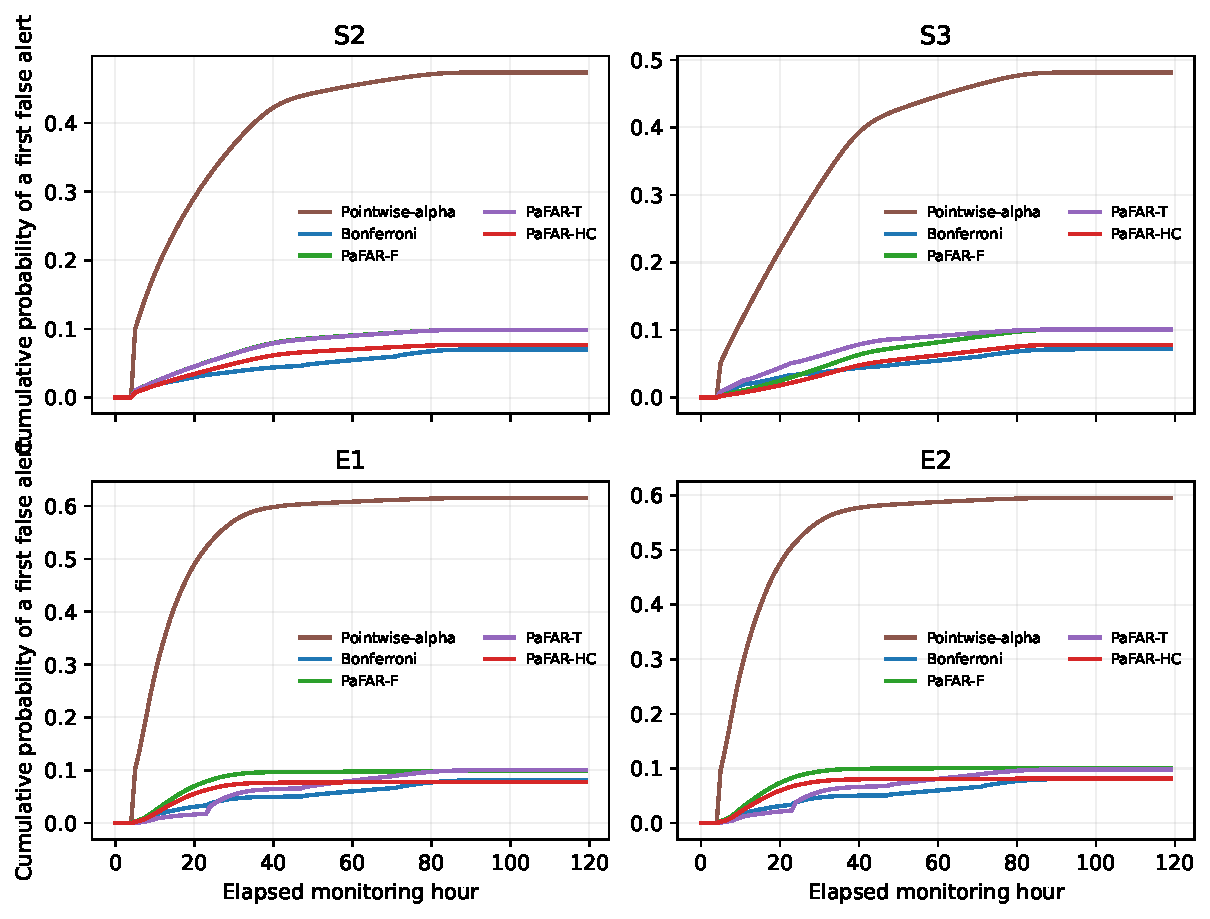
\includegraphics[width=\textwidth]{figure2_cumulative_false_alert.pdf}
\caption{Mean cumulative probability of a first false alert by elapsed monitoring hour at $\alpha=0.10$. Curves use only methods defined for each displayed primary scenario.}
\label{fig:pfa-cumulative}
\end{figure}

\begin{figure}[tbp]
\centering
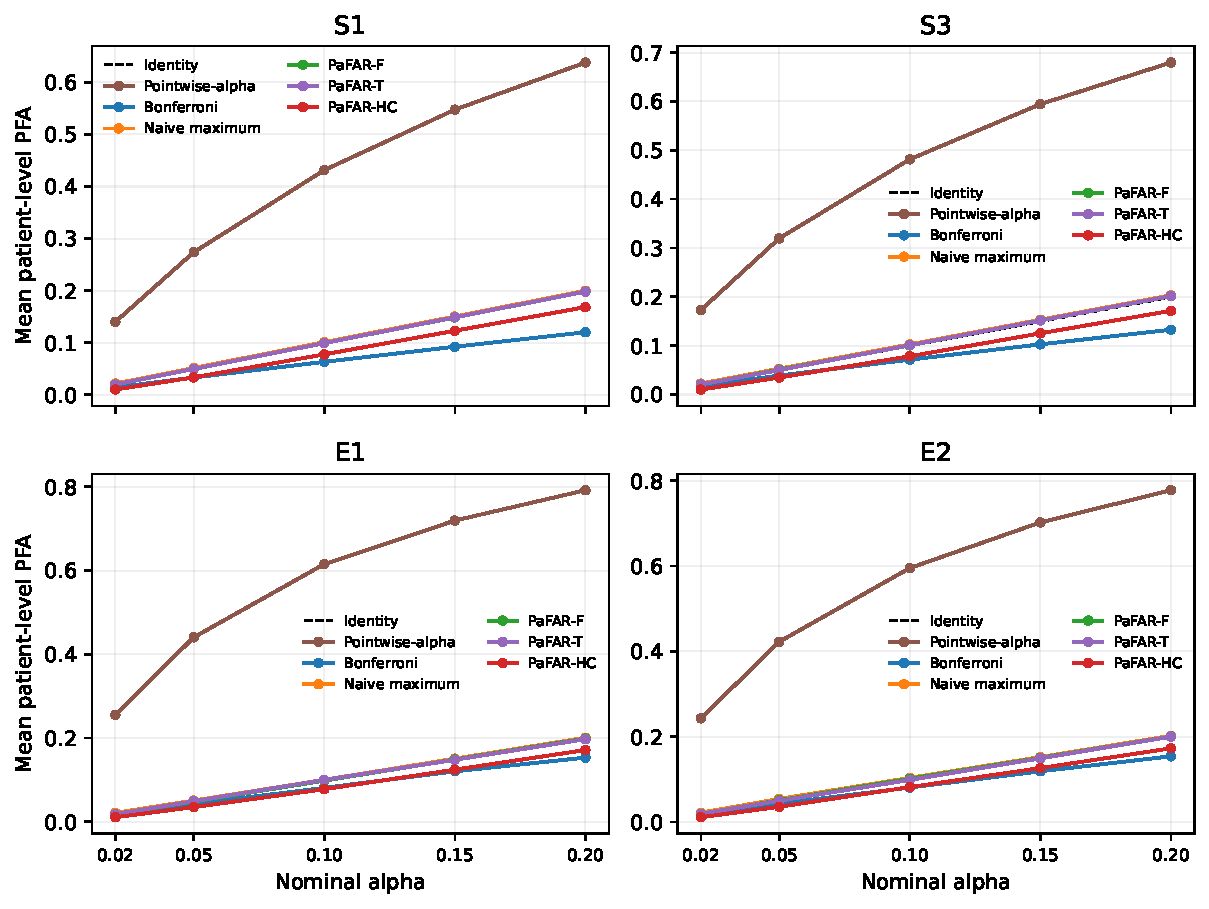
\includegraphics[width=\textwidth]{figure3_pfa_reliability.pdf}
\caption{Mean patient-level PFA over the prespecified reliability grid. The five operating points within a scenario reuse the same primary replicate data and differ only in the recomputed threshold.}
\label{fig:pfa-reliability}
\end{figure}

\subsubsection{End-to-end irregular-EHR performance}

The locked XGBoost learner had mean AUROC 0.716 and trapezoidal PR-AUC 0.097 in E1 and mean AUROC 0.707 and trapezoidal PR-AUC 0.096 in E2; no learner fit failed. These threshold-free measures describe hour-level score discrimination and are not PaFAR operating metrics. Fixed 0.5 produced patient-level PFA 0.751 and 0.733 in E1 and E2, while Youden produced 0.876 and 0.868. Pointwise-alpha PFA remained high at 0.615 and 0.595. PaFAR-F reduced these values to 0.098 and 0.101, but its mean $\Sens_3$ was 0.035 and 0.038. Table~\ref{tab:exp2-primary} reports the selected end-to-end operating summaries; learner metrics are reported once per fitted score generator in Table~\ref{tab:learner-metrics}.

\begin{table}[tbp]
\centering
\caption{Experiment II end-to-end XGBoost results at $\alpha=0.10$.}
\label{tab:exp2-primary}
\small
\setlength{\tabcolsep}{3.5pt}
\resizebox{\linewidth}{!}{%
\begin{tabular}{llrrrrrr}
\toprule
Scenario & Method & PFA & Sens3 & Premature & Median lead & PPV3 & Threshold SD \\
\midrule
E1 & Youden & 0.876 (0.008) & 0.093 (0.003) & 0.800 (0.009) & 3.72 (0.09) & 0.011 (0.000) & 0.049 \\
E1 & Pointwise-alpha & 0.615 (0.006) & 0.119 (0.003) & 0.545 (0.006) & 2.75 (0.04) & 0.019 (0.000) & 0.066 \\
E1 & PaFAR-F & 0.098 (0.002) & 0.035 (0.002) & 0.092 (0.003) & 1.96 (0.04) & 0.033 (0.002) & 0.215 \\
E1 & PaFAR-T & 0.100 (0.002) & 0.030 (0.001) & 0.055 (0.002) & 1.91 (0.05) & 0.029 (0.001) & 0.486 \\
E2 & Pointwise-alpha & 0.595 (0.006) & 0.114 (0.003) & 0.525 (0.006) & 2.80 (0.05) & 0.019 (0.000) & 0.070 \\
E2 & PaFAR-F & 0.101 (0.002) & 0.038 (0.002) & 0.094 (0.003) & 2.06 (0.06) & 0.034 (0.002) & 0.239 \\
E2 & PaFAR-T & 0.098 (0.001) & 0.031 (0.002) & 0.059 (0.003) & 1.99 (0.05) & 0.029 (0.001) & 0.494 \\
E2 & PaFAR-HC & 0.082 (0.001) & 0.032 (0.002) & 0.077 (0.002) & 2.05 (0.05) & 0.035 (0.002) & 0.254 \\
\bottomrule
\end{tabular}
}
\vspace{0.35em}
\begin{minipage}{\linewidth}
\footnotesize
\noindent Entries are Monte Carlo means with Monte Carlo standard errors in parentheses; threshold SD is the across-replicate standard deviation.\par
\noindent Threshold-free AUROC and trapezoidal PR-AUC are reported once per learner in a supplementary table.\par
\noindent Fixed-boundary thresholds and PaFAR-T standardized thresholds are on different numerical scales and are not directly comparable.\par
\end{minipage}
\end{table}


\subsubsection{Time-adaptive standardization}

In S3, where elapsed-time drift was explicit, PaFAR-T reduced descriptive long-stay PFA from 0.181 for PaFAR-F to 0.146 while leaving overall PFA essentially unchanged (0.101 for both after rounding). Mean $\Sens_3$ increased from 0.179 to 0.183. The paired PaFAR-T-minus-PaFAR-F difference in long-stay PFA was $-0.0348$ with paired Monte Carlo SE 0.0008, whereas the overall-PFA difference was 0.0002 with paired Monte Carlo SE 0.0004.

This pattern did not generalize to the learned-score settings. In E1/E2, PaFAR-T had slightly lower $\Sens_3$ than PaFAR-F (0.030 versus 0.035 and 0.031 versus 0.038) and higher descriptive long-stay PFA (0.186 versus 0.104 and 0.172 versus 0.107). XGBoost already used elapsed time, measurement counts, and missingness features, which may have absorbed part of the time structure. Thus the prespecified time template changes efficiency but is not uniformly efficiency-improving; PaFAR-F or PaFAR-T must be chosen before test outcomes are examined. Figure~\ref{fig:sens-pfa-tradeoff} displays the corresponding PFA--$\Sens_3$ operating points.

\begin{figure}[tbp]
\centering
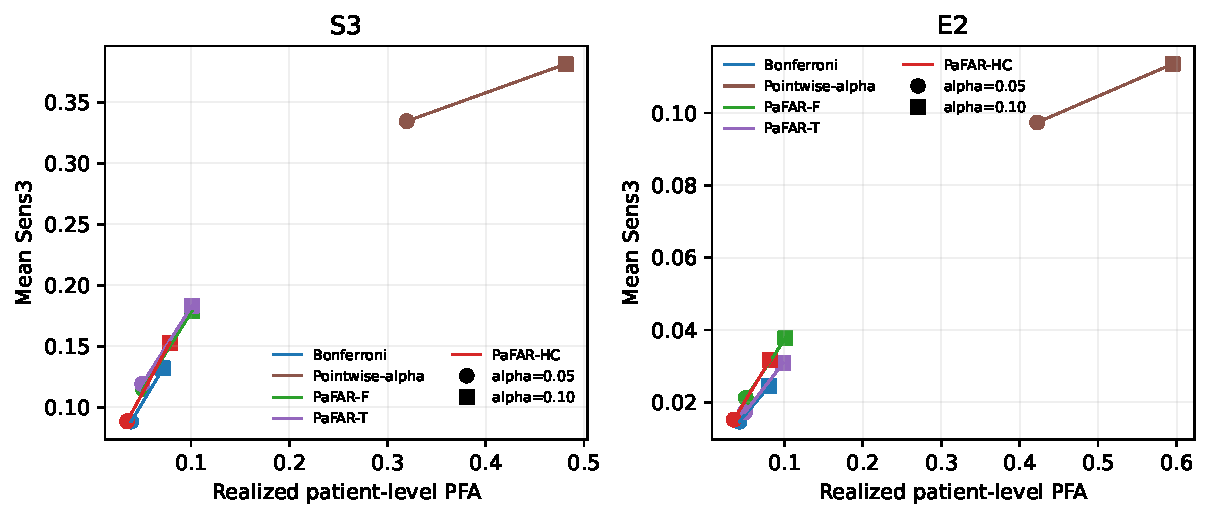
\includegraphics[width=\textwidth]{figure4_sens3_vs_pfa.pdf}
\caption{Mean $\Sens_3$ versus realized patient-level PFA at $\alpha=0.05$ and $0.10$. Marker shape distinguishes the two operating levels, and thin lines connect operating points for the same method.}
\label{fig:sens-pfa-tradeoff}
\end{figure}

\subsubsection{High-confidence conditional control}

At $\alpha=0.10$ and $\delta=0.05$, the fraction of PaFAR-HC calibration replicates whose independent-oracle conditional PFA exceeded $\alpha$ was 0.040 in S1, 0.032 in S2, and 0.048 in S3. Combining the prespecified target-calibration sizes, the corresponding frequency for local S4 PaFAR-HC was 0.038. These frequencies are consistent with the tolerance-limit guarantee and were accompanied by lower sensitivity than PaFAR-F. By contrast, transferring the source S4 PaFAR-HC threshold unchanged yielded an exceedance frequency of 1.000 at $\alpha=0.10$. That source threshold is not protected after the target distribution changes; its failure is therefore not a counterexample to Theorem~\ref{thm:hc}. Figure~\ref{fig:conditional-pfa} uses the independent Experiment I oracle to show the distribution of conditional PFA, with local S4 methods fixed at target $m_0=500$.

\begin{figure}[tbp]
\centering
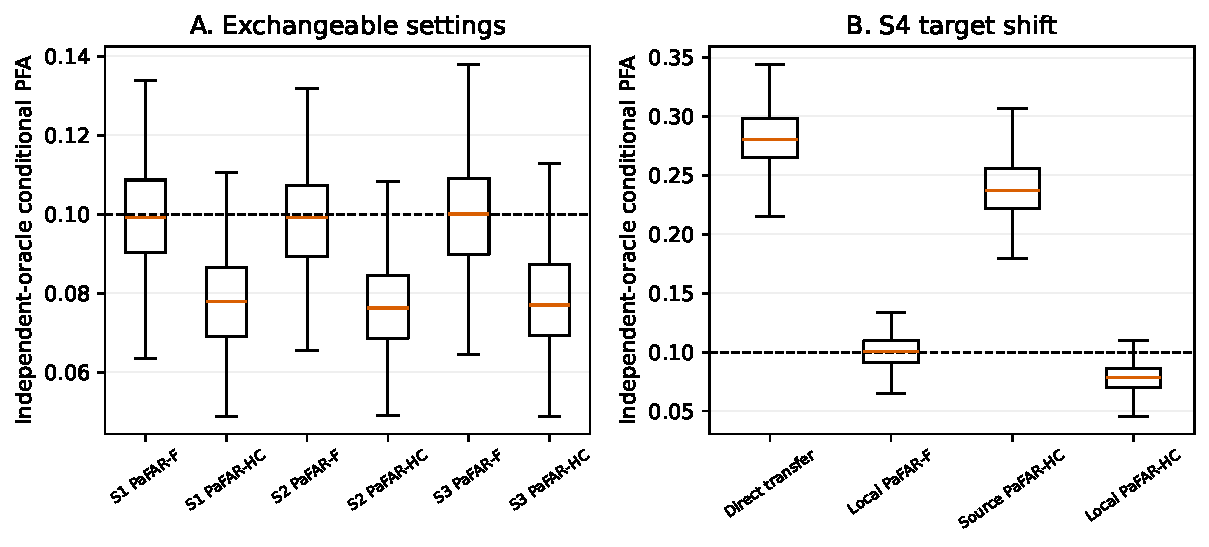
\includegraphics[width=\textwidth]{figure5_conditional_pfa.pdf}
\caption{Independent-oracle conditional PFA at $\alpha=0.10$. Panel A compares PaFAR-F and PaFAR-HC in exchangeable Experiment I settings; Panel B contrasts source transfer with local S4 recalibration at target $m_0=500$. The dashed line is 0.10.}
\label{fig:conditional-pfa}
\end{figure}

\subsubsection{Target-site recalibration}

Direct source transfer was unreliable under both simulated site shifts. Its target PFA was 0.280 in S4 and 0.136 in E3. Re-estimating only the scalar PaFAR-F threshold from 500 target non-events reduced PFA to 0.100 in each experiment. The paired local-minus-direct PFA differences were $-0.1802$ (paired Monte Carlo SE 0.0013) in S4 and $-0.0363$ (paired Monte Carlo SE 0.0035) in E3. The apparently higher $\Sens_3$ of direct transfer accompanied excess false-alert risk and is not an efficiency advantage at equal reliability. The learner and source-fitted time template remained frozen during local recalibration; increasing target $m_0$ primarily reduced threshold variability rather than changing the method. Table~\ref{tab:target-recalibration} and Figure~\ref{fig:target-recalibration} summarize these results.

\input{generated_tables/table5_target_shift.tex}

\begin{figure}[tbp]
\centering
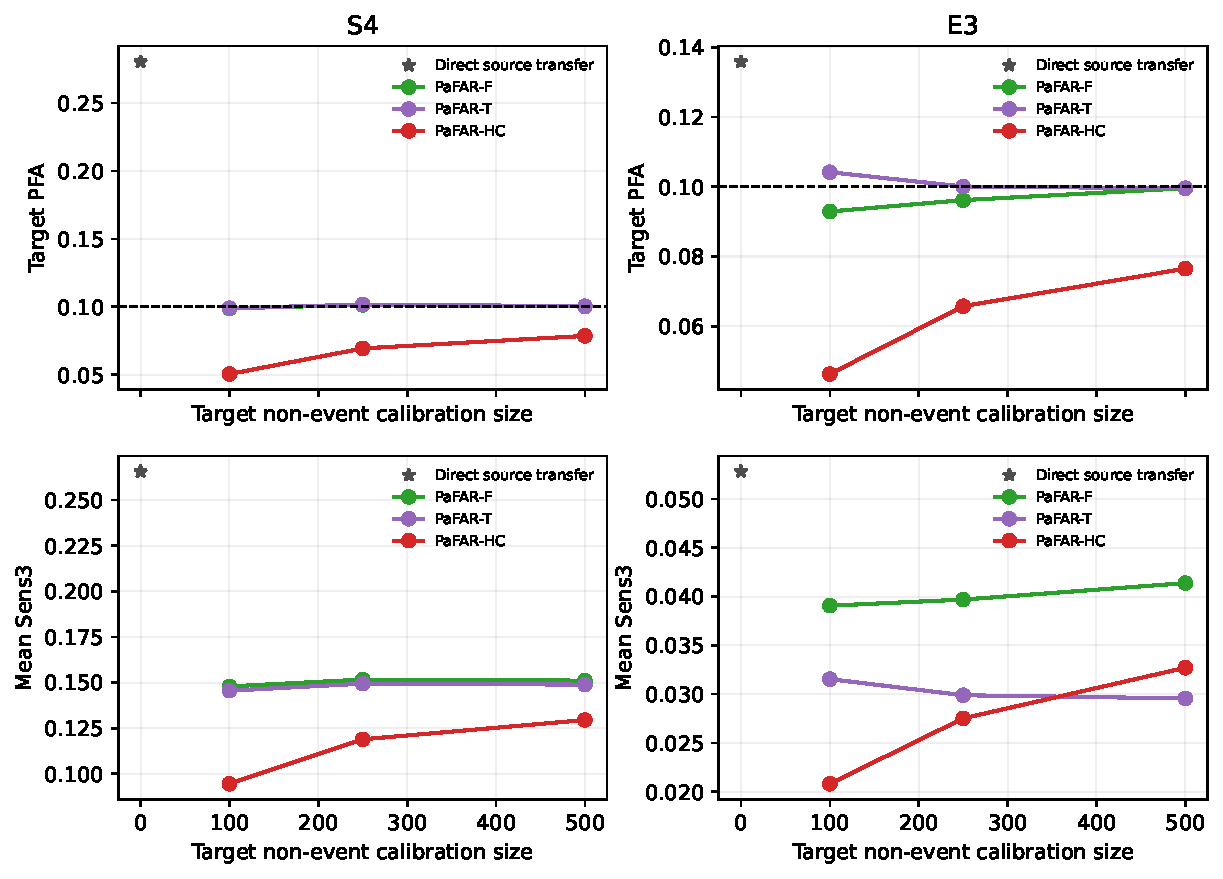
\includegraphics[width=\textwidth]{figure6_target_recalibration.pdf}
\caption{Target PFA and mean $\Sens_3$ before and after local scalar-threshold recalibration. Direct source transfer is the $m_0=0$ reference; local PaFAR-F, PaFAR-T, and PaFAR-HC use nested target non-event prefixes.}
\label{fig:target-recalibration}
\end{figure}

\subsubsection{Reliability--efficiency trade-off}

In the end-to-end simulations, PaFAR-F operated near patient PFA 0.10 but mean $\Sens_3$ was only 0.035 in E1, 0.038 in E2, and 0.041 after local E3 recalibration with $m_0=500$. E3 learner AUROC was 0.723 and trapezoidal PR-AUC was 0.105, yet a trajectory-maximum threshold is more stringent than hour-level discrimination. PaFAR cannot create signal absent from the learner. The low early sensitivity therefore quantifies a substantive reliability--efficiency cost under strict episode-level control, not a failure of the calibration theorem.

\FloatBarrier
\section{Planned PhysioNet 2019 analysis}\label{sec:realdata}

The real-data analysis is specified here as the next application and is not included in the present simulation results.

\subsection{Data source and target task}

The application uses the public training component of the PhysioNet/Computing in Cardiology Challenge 2019 \citep{reyna2019physionet,reyna2020early}. It contains 40,336 ICU patient records from two public hospital-system data sets: 20,336 in set A and 20,000 in set B. Each patient file is organized on an hourly grid and contains 40 predictor variables---vital signs, laboratory measurements, demographics, hospital-admission timing, and ICU length of stay---plus the shifted \texttt{SepsisLabel}. Although the decision grid is hourly, most clinical variables are measured irregularly and contain substantial missingness.

The prediction target is sepsis onset during the next six hours. For an event patient, the onset time is reconstructed as six hours after the first positive shifted label, following the challenge definition. Event records whose first observed hour is already positive are treated as left-truncated and excluded from the primary analysis because the beginning of the warning window cannot be reconstructed reliably.

The primary monitoring protocol is landmarked at six ICU hours: a patient enters the monitoring cohort only if the record is still active at $t_{\min}=6$, a fact known at cohort entry. Monitoring then ends at the earlier of sepsis onset, discharge from the observed episode, or 168 ICU hours. Caps of 96 and 120 hours and the uncapped observed episode are sensitivity analyses. Let $L_i^{\mathrm{ok}}=1$ indicate that an event onset is reconstructable and that the record is not left-truncated. Define the primary landmark cohort
\begin{equation}
\mathcal A_{\mathrm{pri}}=
\{i:H_i\ge t_{\min},D_i=0\}
\cup
\{i:H_i\ge t_{\min},D_i=1,T_i>t_{\min},L_i^{\mathrm{ok}}=1\}.
\label{eq:primary-cohort}
\end{equation}
All primary training, validation, calibration, and test splits are drawn from $\mathcal A_{\mathrm{pri}}$. Patient PFA uses every non-event test patient in this cohort. The denominator of $\Sens_{\ell}$ contains only its event patients with $\calW_{i,\ell}\ne\varnothing$; in particular, $\Sens_3$ requires an eligible time between six and three hours before onset. PPV and alert burden use the full cohort: an alerted event patient who is not evaluable for $\Sens_3$, or whose first alert is premature, remains in the alert denominator but is not a valid $\operatorname{PPV}_3$ detection. Median lead time uses only valid $\Sens_0$ detections. Patients who never reach the landmark have no eligible monitoring time and are outside the primary cohort; their counts are displayed in the cohort flow diagram. A sensitivity analysis that includes them with trajectory score $-\infty$ reports PFA over all recorded ICU episodes. All exclusions and metric-specific denominator counts are reported.

\subsection{Preprocessing and leakage prevention}

Patients, rather than hours, are the units of data splitting. Training-set medians and categorical encodings are estimated once and then applied unchanged to validation, calibration, and test patients. Hospital source is included as a predictor only in the pooled internal analysis; it is omitted from a source-only transfer model because the target-hospital category is not observed during source training. The causal features in \Cref{sec:learner} are recomputed independently within each split. No clinical variable is backfilled from a future measurement. Reconstructed onset, final length of stay, and future measurement frequency are not used as predictors. Elapsed ICU time and information observed up to the current hour are permitted.

The primary XGBoost model is selected by the validation protocol in \Cref{sec:learner}. The three-hour causal score average is fixed before final calibration. PaFAR-T uses the pooled validation non-events and time bins in \eqref{eq:time-bins}; bins with fewer than 50 contributing validation non-events are merged according to the rule in \Cref{subsec:adaptive}. The completed learner, feature map, smoother, and adaptive template are locked before any calibration maxima are computed. Hospital-specific threshold calibration may then be performed on the locked common score map without refitting the learner or template.

\subsection{Internal evaluation}

For the internal analysis, patients in $\mathcal A_{\mathrm{pri}}$ are stratified by hospital set and event status and allocated to 50\% training, 15\% validation, 15\% calibration, and 20\% test sets. For each candidate hyperparameter configuration, a single XGBoost learner is fitted using only the pooled training patients from hospital sets A and B. Hyperparameters and the number of boosting rounds are selected using only the pooled validation patients, with early stopping performed on the validation set. Hospital source is included as a predictor. The selected learner is then frozen; no refitting on the union of the training and validation sets is performed in the primary implementation. After learner selection, the PaFAR-T template is estimated from the pooled validation non-events and frozen before any calibration trajectory is examined. One prespecified seed defines the primary analysis and the XGBoost grid is run only for this split. Nine additional prespecified seeds assess split sensitivity in the supplement: within each new split, the learner is fitted on the pooled training patients using the hyperparameter configuration selected in the primary analysis, early stopping is performed on the pooled validation patients, and template estimation and threshold calibration are rerun in their designated splits.

For the primary reliability analysis, all calibration-based rules---pointwise-$\alpha$, Bonferroni conformal, naive maximum, PaFAR-F, PaFAR-T, and PaFAR-HC---are calibrated separately within hospital sets A and B using only their non-event calibration patients. Each test patient is evaluated with the threshold from that patient's hospital. For PaFAR methods, \Cref{thm:stratum} then gives hospital-specific control and therefore control of the overall hospital mixture. A single threshold estimated from pooled calibration non-events is reported only as a secondary sensitivity analysis. Fixed 0.5 and the pooled-validation Youden threshold remain conventional uncalibrated baselines. The primary operating points are $\alpha=0.05$ and $0.10$; PaFAR-HC uses $\delta=0.05$. Every comparison uses the same locked XGBoost trajectories. A regularized logistic-regression score generator is optional as a secondary robustness analysis.

\subsection{Cross-hospital transfer and local recalibration}

External-style analyses are run in both directions, A$\rightarrow$B and B$\rightarrow$A. For each direction, a fixed source-hospital split allocates 60\% of source patients to training, 20\% to validation, and 20\% to calibration, stratified by event status. The feature pipeline, base learner, PaFAR-T template, and source threshold are developed once using these source data only. Two deployment strategies are compared:
\begin{enumerate}
    \item \textbf{Direct transfer}: apply the source patient-level threshold unchanged at the target hospital.
    \item \textbf{Local recalibration}: keep the source learner, feature map, smoother, and PaFAR-T template fixed, and recompute only the scalar patient-level threshold using $m_{0B}\in\{100,250,500,1000\}$ historical target-hospital non-event patients.
\end{enumerate}
One prespecified target partition defines the primary analysis: 50\% of target patients form a test set stratified by event status and the remaining 50\% form a calibration reservoir. The target non-event calibration samples of sizes $100$, $250$, $500$, and $1000$ are nested draws from that reservoir; reservoir event patients are unused. Direct transfer and every local-recalibration strategy are evaluated on the same primary target test patients, and the fixed source model is not refitted. Forty-nine additional prespecified target partitions repeat this allocation only to assess split sensitivity. Their overlapping results are summarized by the median, interquartile range, minimum, and maximum and are not treated as independent replications for standard errors or inferential intervals. Target event patients are never used to compute the false-alarm threshold.

\subsection{Outcomes and uncertainty summaries}

The primary test outcome is the proportion of non-event patients receiving at least one formal alert. In the hospital-specific internal analysis, each hospital's PFA is accompanied by a two-sided 95\% exact binomial interval and a one-sided 95\% exact upper bound. The overall PFA is the observed-hospital-mixture weighted average of the two hospital-specific proportions and receives a stratified patient-bootstrap interval rather than a homogeneous-binomial interval. In each cross-hospital target analysis, which contains one target hospital, the corresponding exact binomial intervals are reported. These intervals describe realized test performance; they are not substituted for the finite-sample calibration theorem. The main detection outcome is $\Sens_3$, followed by $\Sens_0$. Secondary outcomes are premature-alert probability, median valid lead time, PPV, alerts per 100 patient-days, weighted trapezoidal PR-AUC, AUROC, and the official challenge utility.

The challenge utility is an auxiliary benchmark and is not used for learner or threshold selection. Define the utility evaluation grid
\[
\calI_i^{\mathrm{util}}=\{t\in\calT_i:t_{\min}\le t\le\min(H_i,H_{\max})\},
\]
which, unlike \eqref{eq:monitoring-set}, is not truncated at sepsis onset because the official scorer evaluates every recorded hour. At each $t\in\calI_i^{\mathrm{util}}$, each method outputs its ordinary threshold indicator (for example, $\Ind\{Z_i^{\eta}(t)>c\}$ for PaFAR), and outputs zero outside this grid. The original challenge scoring function is then applied to these hourly binary predictions. This auxiliary calculation does not alter the pre-onset first-alert estimands or the theoretical guarantee.

Pairwise method differences are summarized using 1,000 patient-level bootstrap samples of the fixed primary test set. Entire patient trajectories are resampled; hours are never resampled independently. The internal bootstrap is stratified by hospital and event status, and a cross-hospital target bootstrap is stratified by event status. These intervals condition on the fitted learner, template, and threshold. The nine internal split-sensitivity analyses and 49 additional target partitions are summarized descriptively and are not pooled as independent samples. Subgroup results are descriptive, and no subgroup-specific control is claimed unless that subgroup has its own independently calibrated threshold.

\subsection{Subgroup and duration analyses}

False-alert rates are reported by hospital, sex, age group, available ICU-type indicators, and eligible monitoring-exposure quartile. Except for the primary hospital-specific thresholds, these are descriptive subgroup evaluations unless a separate stratum-specific threshold has been calibrated with adequate non-event sample size. In particular, longest-quartile PFA is not interpreted as a guaranteed level-$\alpha$ quantity. For elapsed time $u$, define
\begin{equation}
\widehat C_{\mathrm{FA}}(u)=\frac{1}{n_0}
\sum_{i:D_i=0}\Ind\{\tau_i\le\min(u,H_i)\},
\label{eq:cumulative-alert}
\end{equation}
which estimates the probability that an observed non-event episode has produced an alert by hour $u$. A complementary analysis conditions on patients still under observation at $u$ to display the effect of selective long stays.

\subsection{Real-data results}

The locked primary cohort contained 39,895 patients and 1,448,195 patient-hour
rows across the two hospitals.  At $\alpha=0.10$, hospital-specific PaFAR-F
calibration yielded an overall patient PFA of 0.102 (95\% bootstrap interval
0.096--0.109) and $\Sens_3=0.061$.  Pointwise-$\alpha$ calibration instead
yielded PFA 0.426, illustrating the accumulation of repeated false-alert
opportunities.  In transfer, the frozen A-to-B source threshold was
conservative (PFA 0.032), whereas the frozen B-to-A threshold was
anti-conservative (PFA 0.315).  Local scalar recalibration moved the target
PFA toward 0.10 without refitting the learner.

\input{generated_tables/table6_physionet_internal.tex}

\begin{table}[!htbp]
\centering
\caption{Cross-hospital deployment and local scalar-threshold recalibration at $\alpha=0.10$.}
\label{tab:real-external}
\resizebox{\linewidth}{!}{%
\begin{tabular}{llccccc}
\toprule
Direction & Strategy & Target $m_0$ & Target PFA [95\% exact interval] & Sens$_3$ & PPV$_3$ & Utility \\
\midrule
A$\rightarrow$B & Direct source transfer & 0 & 0.032 [0.029, 0.036] & 0.007 & 0.008 & 0.016 \\
A$\rightarrow$B & Local PaFAR-F & 100 & 0.070 [0.065, 0.076] & 0.033 & 0.017 & 0.039 \\
A$\rightarrow$B & Local PaFAR-F & 250 & 0.084 [0.078, 0.090] & 0.033 & 0.014 & 0.045 \\
A$\rightarrow$B & Local PaFAR-F & 500 & 0.082 [0.076, 0.087] & 0.033 & 0.015 & 0.043 \\
A$\rightarrow$B & Local PaFAR-F & 1000 & 0.094 [0.088, 0.100] & 0.035 & 0.014 & 0.050 \\
A$\rightarrow$B & Local PaFAR-T & 500 & 0.086 [0.081, 0.092] & 0.033 & 0.013 & 0.177 \\
A$\rightarrow$B & Local PaFAR-HC & 500 & 0.064 [0.059, 0.069] & 0.028 & 0.015 & 0.035 \\
B$\rightarrow$A & Direct source transfer & 0 & 0.315 [0.306, 0.325] & 0.062 & 0.013 & 0.223 \\
B$\rightarrow$A & Local PaFAR-F & 100 & 0.092 [0.086, 0.098] & 0.039 & 0.024 & 0.109 \\
B$\rightarrow$A & Local PaFAR-F & 250 & 0.115 [0.108, 0.121] & 0.043 & 0.022 & 0.124 \\
B$\rightarrow$A & Local PaFAR-F & 500 & 0.127 [0.121, 0.134] & 0.044 & 0.021 & 0.131 \\
B$\rightarrow$A & Local PaFAR-F & 1000 & 0.102 [0.096, 0.108] & 0.044 & 0.025 & 0.117 \\
B$\rightarrow$A & Local PaFAR-T & 500 & 0.114 [0.108, 0.121] & 0.040 & 0.022 & 0.100 \\
B$\rightarrow$A & Local PaFAR-HC & 500 & 0.093 [0.087, 0.099] & 0.039 & 0.024 & 0.110 \\
\bottomrule
\end{tabular}%
}
\begin{minipage}{0.98\linewidth}\footnotesize Target PFA intervals are two-sided Clopper--Pearson intervals. Direct transfer uses the frozen source PaFAR-F threshold; local methods change only the scalar threshold.\end{minipage}
\end{table}


\begin{figure}[!htbp]
\centering
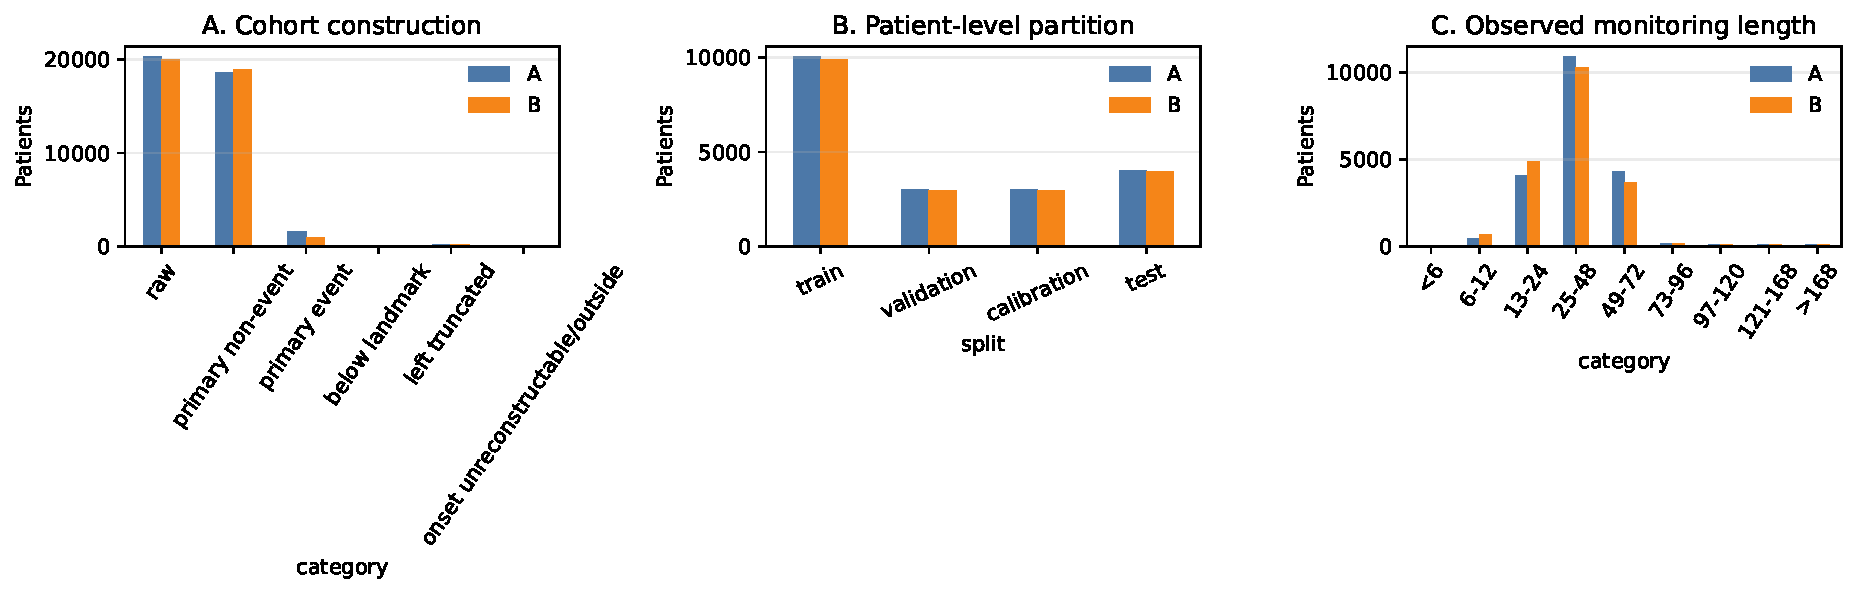
\includegraphics[width=\linewidth]{figure7_cohort_flow.pdf}
\caption{Cohort construction, patient-level partitioning, and observed monitoring length.}
\label{fig:real-cohort-flow}
\end{figure}

\begin{figure}[!htbp]
\centering
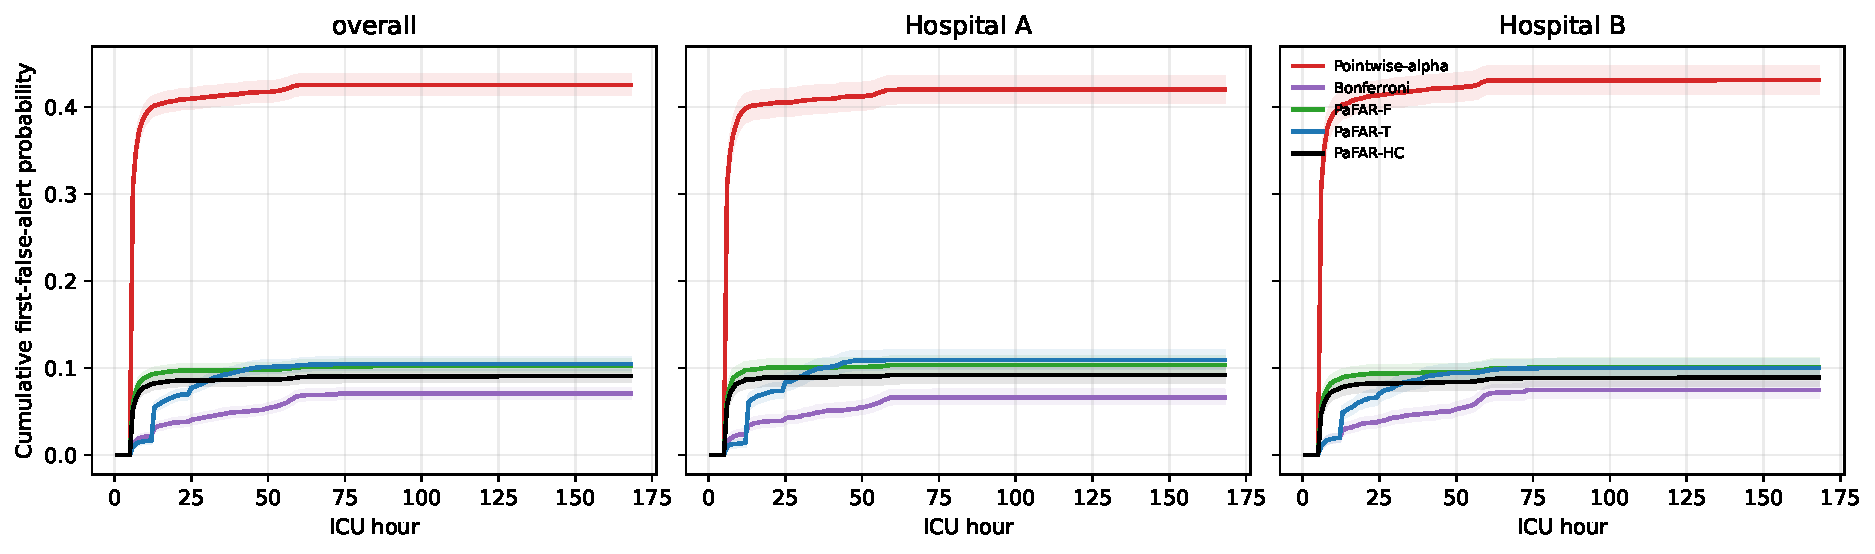
\includegraphics[width=\linewidth]{figure8_realdata_false_alert.pdf}
\caption{Cumulative patient-level false-alert probability in the internal PhysioNet test set at $\alpha=0.10$, with hospital-stratified whole-patient bootstrap bands.}
\label{fig:real-cumulative-fa}
\end{figure}

\begin{figure}[!htbp]
\centering
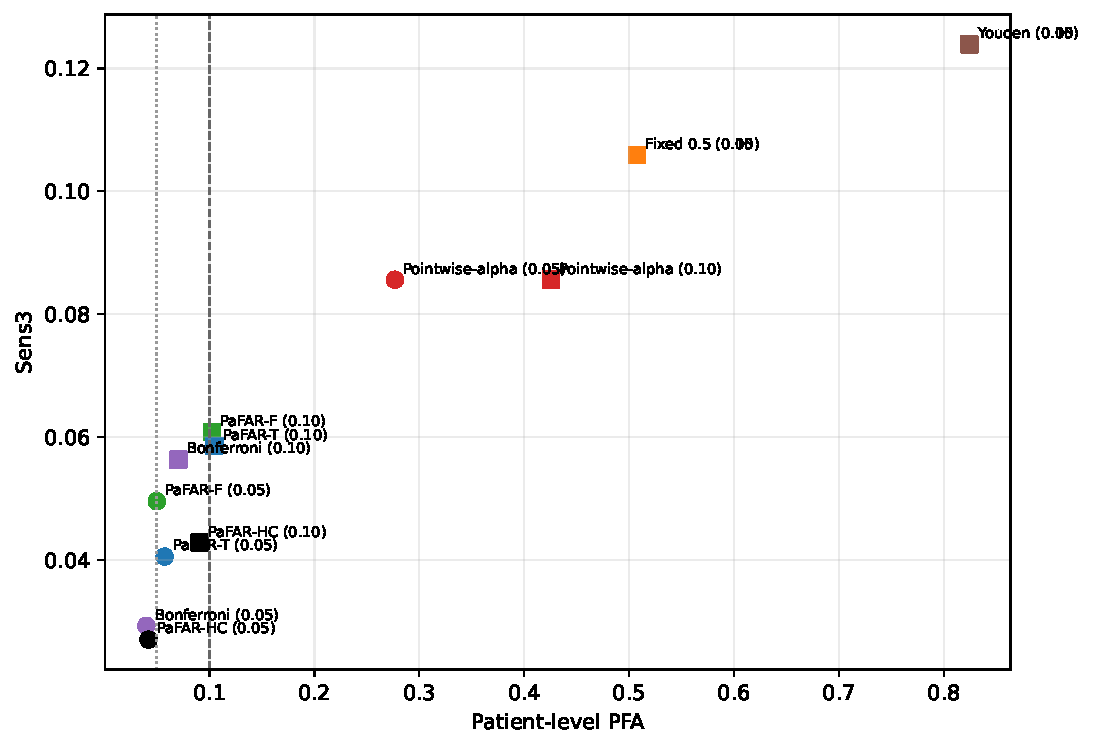
\includegraphics[width=0.82\linewidth]{figure9_realdata_tradeoff.pdf}
\caption{Three-hour-lead sensitivity versus patient-level false-alarm probability at the calibrated real-data operating points.}
\label{fig:real-tradeoff}
\end{figure}

\begin{figure}[!htbp]
\centering
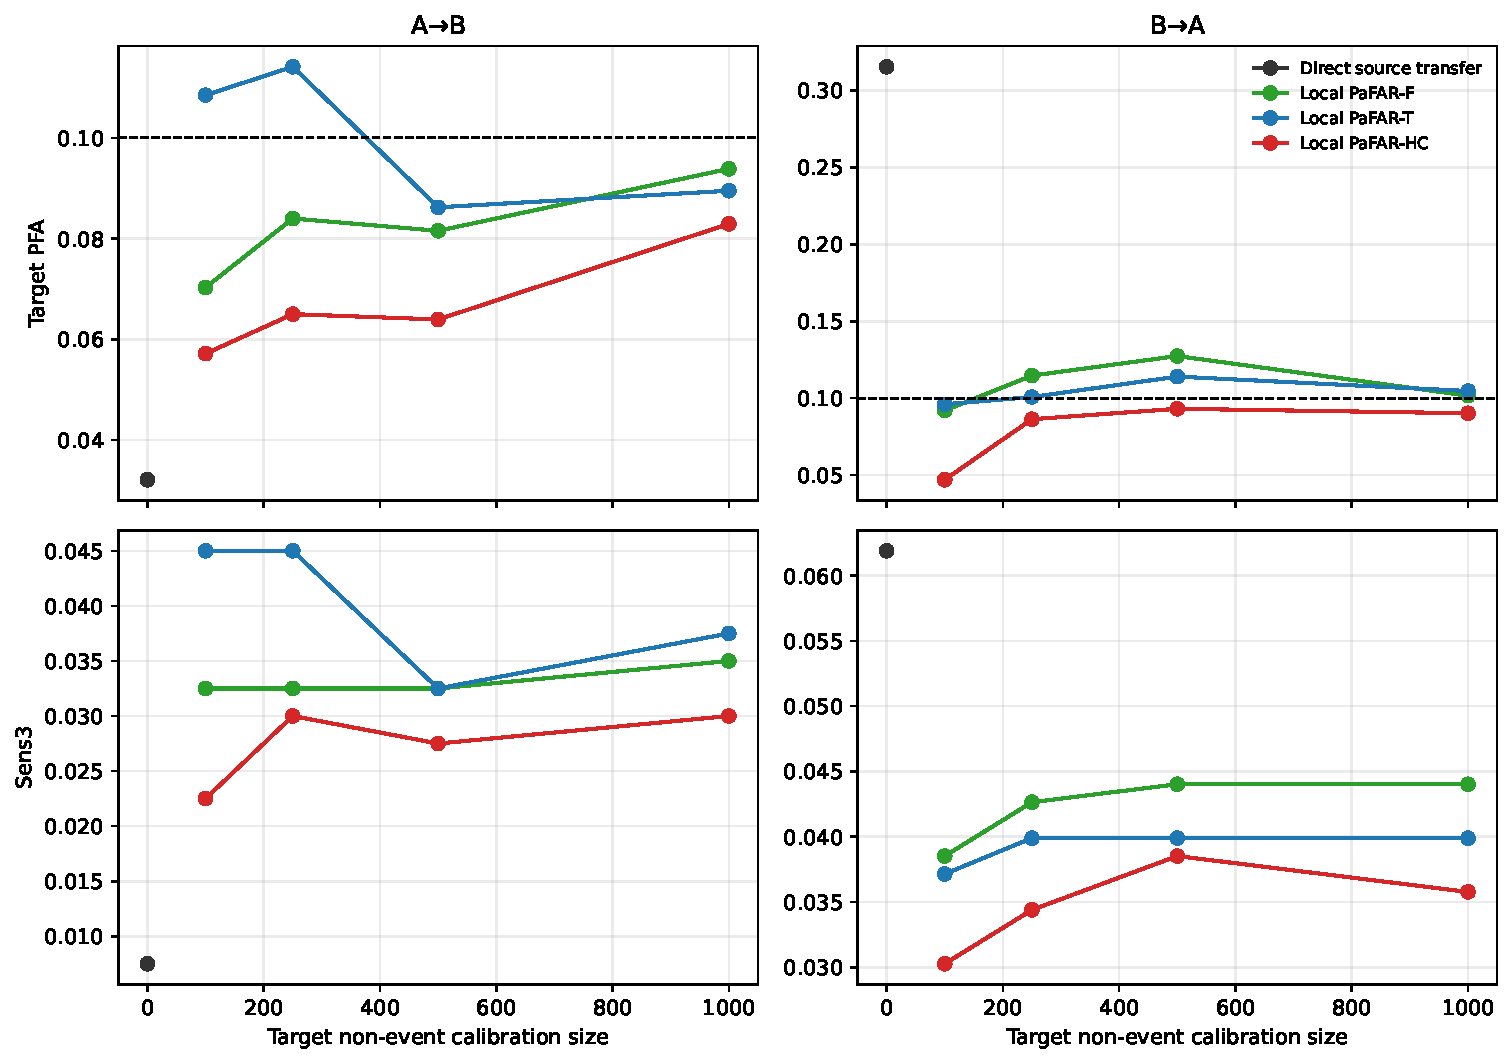
\includegraphics[width=0.92\linewidth]{figure10_cross_hospital.pdf}
\caption{Cross-hospital target PFA and three-hour-lead sensitivity before and after local scalar-threshold recalibration.}
\label{fig:real-transfer}
\end{figure}

\section{Discussion}\label{sec:discussion}

PaFAR changes the reliability unit from an individual prediction time to a complete patient monitoring episode. The completed primary simulations supported the finite-sample marginal statement in its intended exchangeable settings: PaFAR-F and PaFAR-T mean PFA closely tracked $\alpha_{m_0}$ across the five-level reliability grid. This contrasts with pointwise-alpha calibration, whose patient-level PFA at nominal 0.10 ranged from approximately 0.43 to 0.62. The cumulative-alert curves make the operational distinction concrete: pointwise specificity did not prevent false alerts from accumulating over a trajectory.

The method is intentionally model agnostic and does not improve score discrimination. The end-to-end learners achieved AUROC approximately 0.71--0.72, but strict trajectory-maximum calibration left mean $\Sens_3$ near 0.03--0.04 in E1--E3. A more informative learner may preserve more early sensitivity at the same PFA, but PaFAR cannot create signal that the learner does not contain. The observed loss is therefore a substantive reliability--efficiency trade-off. It should not be described as evidence of high clinical sensitivity or as a failure of the calibration theorem.

PaFAR-HC addressed a different target from marginal PaFAR. In the exchangeable score-process scenarios, its independent-oracle conditional exceedance frequency at $\delta=0.05$ was close to the prespecified level, but the resulting thresholds were more conservative and sensitivity was lower. The marginal and tolerance-limit guarantees should therefore not be treated as synonyms. They answer different deployment questions and impose different efficiency costs.

The time-adaptive result was similarly qualified. PaFAR-T reduced the long-stay PFA imbalance in S3 without materially changing overall PFA and slightly increased $\Sens_3$. It did not improve efficiency in E1 or E2, where $\Sens_3$ was slightly lower and descriptive long-stay PFA was higher than for PaFAR-F. The EHR learner already incorporated elapsed time, measurement counts, and missingness features. The fixed and time-adaptive score definitions must consequently be prespecified rather than selected after observing test performance.

Distribution shift exposed the boundary of the theory. Direct source-threshold transfer yielded PFA 0.280 in S4 and 0.136 in E3, whereas local target-site recalibration of the scalar threshold restored PFA to approximately 0.10. The higher sensitivity under direct transfer occurred at substantially greater false-alert risk and was not an equal-reliability advantage. Theorems~\ref{thm:marginal}--\ref{thm:hc} apply only under their stated exchangeability or i.i.d. conditions; source-transfer failure after a distribution change does not contradict them.

Several limitations remain. Exchangeability may fail under hospital shift, temporal drift, changed measurement policies, or model-driven clinical interventions. Target-site recalibration is valid only when local calibration patients represent future target patients. The guarantee is conditional on the recorded non-event label, so undetected events and label error change the target population. Retrospective evaluation cannot capture alert-induced changes in testing, treatment, discharge, or event ascertainment. Marginal control also does not imply equal subgroup control. Duration heterogeneity may yield a higher conditional false-alert probability among long episodes, while a single globally calibrated threshold can reduce sensitivity among shorter episodes. The prespecified cap, descriptive duration analyses, time-adaptive boundary, and hospital-specific calibration address selected aspects of this heterogeneity but do not provide duration-conditional control.

The contribution should therefore be stated narrowly. The simulations establish computational feasibility and clarify reliability behavior under controlled mechanisms, and the retrospective PhysioNet analysis evaluates the locked procedure under two observed hospital domains; neither demonstrates prospective clinical effectiveness. Clinical usefulness still requires careful label and subgroup audits and prospective evaluation under intervention feedback.

\section{Conclusion}

PaFAR is a lightweight patient-trajectory reliability layer for repeated black-box scores. The primary simulations supported its finite-sample marginal control under exchangeability and showed that pointwise calibration can produce severe patient-level false-alert accumulation. The high-confidence threshold reduced conditional exceedance probability but was more conservative. Under both simulated and observed hospital shift, direct source-threshold transfer could miss the target, whereas local recalibration changed only the scalar threshold and moved patient-level PFA toward the target without refitting the learner. Strict control could substantially reduce early sensitivity, so reliability and detection efficiency must be reported together. These results do not imply that PaFAR improves discrimination, that PaFAR-T uniformly improves efficiency, or that the method has been clinically validated. Prospective evaluation remains the next empirical step.
\appendix

\section{Proofs}\label{app:proofs}

\subsection{Proof of Theorem~\ref{thm:marginal}}

\begin{proof}
Condition on $\calF_{\mathrm{fit}}$ and on the observed calibration non-event count $m_0$. Under \Cref{ass:frozen,ass:stable-episode}, the same measurable map
\[
\mathcal S_{\eta}(\mathcal O_i)
=\max_{t\in\calI_i}Z_i^{\eta}(t)
\]
is applied to every calibration and deployment trajectory. By \Cref{ass:exchangeability}, the scalar scores
\[
M_1^{\eta},\ldots,M_{m_0}^{\eta},M_{\mathrm{new}}^{\eta}
\]
are therefore exchangeable.

To handle ties, let $U_1,\ldots,U_{m_0},U_{\mathrm{new}}$ be independent $\operatorname{Uniform}(0,1)$ variables, independent of all trajectory scores. Order the pairs $(M_i^{\eta},U_i)$ lexicographically. The pairs are exchangeable and almost surely have no ties, so the lexicographic rank
\[
R_{\mathrm{new}}
=1+\sum_{i=1}^{m_0}
\Ind\{(M_i^{\eta},U_i)<_{\mathrm{lex}}
(M_{\mathrm{new}}^{\eta},U_{\mathrm{new}})\}
\]
is uniform on $\{1,\ldots,m_0+1\}$.

Let $k=k_{\alpha}(m_0)$. If $k=m_0+1$, then the augmented threshold is $+\infty$ and the exceedance probability is zero. Suppose instead that $k\le m_0$. If $M_{\mathrm{new}}^{\eta}>M_{(k)}^{\eta}$, then at least $k$ calibration scores are strictly smaller than $M_{\mathrm{new}}^{\eta}$. Hence at least $k$ calibration pairs precede the new pair lexicographically, which implies $R_{\mathrm{new}}>k$. Consequently,
\begin{align*}
\Pp\{M_{\mathrm{new}}^{\eta}>M_{(k)}^{\eta}
\mid D_{\mathrm{new}}=0,\calF_{\mathrm{fit}},m_0\}
&\le \Pp(R_{\mathrm{new}}>k)\\
&=\frac{m_0+1-k}{m_0+1}.
\end{align*}
Together with the $k=m_0+1$ case, the same bound holds for every $m_0\ge0$.

Finally,
\[
k=\left\lceil(m_0+1)(1-\alpha)\right\rceil
\ge(m_0+1)(1-\alpha),
\]
which gives
\[
\frac{m_0+1-k}{m_0+1}\le\alpha.
\]
By \eqref{eq:first-alert} and \eqref{eq:trajectory-score},
\[
\{\exists t\in\calI_{\mathrm{new}}:
Z_{\mathrm{new}}^{\eta}(t)>\widehat c_{\alpha}^{\eta}\}
=\{M_{\mathrm{new}}^{\eta}>\widehat c_{\alpha}^{\eta}\},
\]
so the preceding inequality is exactly \eqref{eq:theorem-marginal}. Monitoring length, missingness, and temporal dependence are components of $\mathcal O_i$; the proof never assumes that decision times within a patient are independent or identically distributed.
\end{proof}

\subsection{Proof of Corollary~\ref{cor:adaptive}}

\begin{proof}
By construction, $\widehat\eta$ is measurable with respect to $\calF_{\mathrm{fit}}$. Conditional on $\calF_{\mathrm{fit}}$, the functions $a_{\widehat\eta}$ and $b_{\widehat\eta}$, the time bins, the smoother, and every other part of the trajectory-score map are fixed. The calibration and deployment scores are therefore obtained by applying one common measurable map to exchangeable non-event trajectories. \Cref{thm:marginal} applies conditionally on $\calF_{\mathrm{fit}}$, proving the result.
\end{proof}

\subsection{Proof of Theorem~\ref{thm:stratum}}

\begin{proof}
Fix a stratum $g$ and condition on $\calF_{\mathrm{fit}}$, $m_{0g}$, $D_{\mathrm{new}}=0$, and $G_{\mathrm{new}}=g$. By assumption, the $m_{0g}$ calibration non-event trajectories in stratum $g$ and the new non-event trajectory in that stratum are exchangeable. Applying the proof of \Cref{thm:marginal} within this conditional population yields
\[
\Pp\{M_{\mathrm{new}}^{\eta}>
\widehat c_{\alpha,g}^{\eta}
\mid D_{\mathrm{new}}=0,G_{\mathrm{new}}=g,
\calF_{\mathrm{fit}},m_{0g}\}
\le\alpha.
\]
The event on the left is equivalent to at least one alert, proving \eqref{eq:stratum-control}. Integrating this conditional inequality over the distribution of $m_{0g}$ gives
\[
\Pp\{\tau_{\mathrm{new}}<\infty
\mid D_{\mathrm{new}}=0,G_{\mathrm{new}}=g,
\calF_{\mathrm{fit}}\}\le\alpha.
\]

If every stratum is calibrated at level $\alpha$, then by the law of total probability,
\begin{align*}
&\Pp\{\tau_{\mathrm{new}}<\infty\mid D_{\mathrm{new}}=0,\calF_{\mathrm{fit}}\}\\
&\quad=\sum_{g=1}^{G}
\Pp\{\tau_{\mathrm{new}}<\infty
\mid D_{\mathrm{new}}=0,G_{\mathrm{new}}=g,
\calF_{\mathrm{fit}}\}
\Pp\{G_{\mathrm{new}}=g\mid D_{\mathrm{new}}=0,\calF_{\mathrm{fit}}\}\\
&\quad\le\sum_{g=1}^{G}\alpha
\Pp\{G_{\mathrm{new}}=g\mid D_{\mathrm{new}}=0,\calF_{\mathrm{fit}}\}
=\alpha.
\end{align*}
\end{proof}

\subsection{Proof of Theorem~\ref{thm:hc}}

\begin{proof}
Condition on $\calF_{\mathrm{fit}}$ and $m_0$, and write $m=m_0$, $q=1-\alpha$, and $k=k_{\alpha,\delta}^{\mathrm{HC}}(m)$. If $k=m+1$, then the threshold is $+\infty$ and the conditional deployment risk is zero, so the result is immediate. Suppose $k\le m$.

Let $F_0$ be the distribution function of a non-event trajectory score and define the generalized $q$-quantile
\[
x_q=\inf\{x:F_0(x)\ge q\}.
\]
For a realized threshold $c$, the conditional false-alarm probability is
\[
r(c)=\Pp(M_{\mathrm{new}}^{\eta}>c\mid D_{\mathrm{new}}=0,\calF_{\mathrm{fit}})
=1-F_0(c).
\]
Therefore,
\[
r\{M_{(k)}^{\eta}\}>\alpha
\quad\Longleftrightarrow\quad
F_0\{M_{(k)}^{\eta}\}<q.
\]
By the definition of $x_q$, the latter event implies $M_{(k)}^{\eta}<x_q$. Let
\[
p_-=F_0(x_q^-)=\Pp(M_i^{\eta}<x_q\mid D_i=0,\calF_{\mathrm{fit}}).
\]
The generalized-quantile definition gives $p_-\le q$. Under \Cref{ass:hc},
\[
N_-=\sum_{i=1}^{m}\Ind(M_i^{\eta}<x_q)
\sim\operatorname{Binomial}(m,p_-).
\]
Moreover, $M_{(k)}^{\eta}<x_q$ if and only if at least $k$ calibration scores are smaller than $x_q$, that is, $N_-\ge k$. Hence
\begin{align*}
\Pp_{\calD_{\mathrm{cal},0}}\!
\left[r\{M_{(k)}^{\eta}\}>\alpha\right]
&\le \Pp\{\operatorname{Binomial}(m,p_-)\ge k\}\\
&\le \Pp\{\operatorname{Binomial}(m,q)\ge k\}\\
&=\sum_{j=k}^{m}\binom{m}{j}q^j(1-q)^{m-j}\\
&\le\delta,
\end{align*}
where the second inequality follows from monotonicity of the binomial upper tail in its success probability, and the last inequality is the definition of $k_{\alpha,\delta}^{\mathrm{HC}}(m)$. This is \eqref{eq:hc-guarantee}. The argument uses $F_0(x_q^-)$ and therefore remains valid when $F_0$ has atoms; continuity and randomized tie breaking are unnecessary.
\end{proof}

\subsection{Calibration-size statements}

For marginal PaFAR, a non-augmented order-statistic threshold is available precisely when
\[
\left\lceil(m_0+1)(1-\alpha)\right\rceil\le m_0.
\]
Because the right-hand side is an integer, this is equivalent to
\[
(m_0+1)(1-\alpha)\le m_0
\quad\Longleftrightarrow\quad
m_0+1\ge\frac{1}{\alpha},
\]
which proves \eqref{eq:min-cal-marginal}.

For PaFAR-HC, among the non-augmented order statistics the smallest possible binomial upper tail occurs at $k=m_0$ and equals
\[
\Pp\{\operatorname{Binomial}(m_0,1-\alpha)\ge m_0\}
=(1-\alpha)^{m_0}.
\]
Thus a non-augmented qualifying index exists if and only if $(1-\alpha)^{m_0}\le\delta$. Taking logarithms gives \eqref{eq:hc-min-sample}.

\section{Detailed simulation parameters}\label{app:simulation-parameters}

\begin{longtable}{L{0.27\linewidth}L{0.25\linewidth}L{0.38\linewidth}}
\caption{Primary simulation parameters and one-factor sensitivity values.}\label{tab:sim-parameters}\\
\toprule
Component & Primary value & Sensitivity values or notes \\
\midrule
\endfirsthead
\toprule
Component & Primary value & Sensitivity values or notes \\
\midrule
\endhead
Target patient PFA & $\alpha=0.10$ & Reliability grid $0.02,0.05,0.10,0.15,0.20$ within each shared primary replicate; thresholds only are recomputed. \\
HC confidence & $\delta=0.05$ & $0.10$ optional sensitivity. \\
Score-process calibration non-events & $m_0=500$ & $100,250,1000$ in S2 and S3. \\
Event prevalence & $\pi=0.10$ & $0.05$ obtained only by reweighting PPV and alert burden; class-conditional metrics and thresholds are unchanged. \\
Simulation monitoring cap & $H_{\max}=120$ h & 72 h short-stay setting. \\
Real-data monitoring cap & 168 h & 96 h, 120 h, and uncapped. \\
Burn-in & $t_{\min}=6$ h & 0 h and 12 h. \\
Admissible warning window & $W_{\max}=h=6$ h & Report minimum lead $\ell=3,0$ h. \\
Score signal & $\Delta=1.5$ & $1.0$ weak signal. \\
EHR background process & AR coefficient $0.85$, innovation SD $0.35$ & Initialized at stationarity; frailty loading $0.40$. \\
EHR severity signal & $\Delta_S=1.0$ & $0.65$ weak signal. \\
EHR event intercept & $\beta_{\pi,0}=-2.3845$ & Gives marginal event prevalence 0.10. \\
Patient random-effect SD & $\sigma_b=0.45$ & Fixed in the primary manuscript. \\
Score AR correlation & $\rho=0.80$ & Fixed in the primary manuscript. \\
Score AR marginal SD & $\sigma_{E,A}=0.55$ & Site B multiplies by 1.10. \\
Score-process intercept & $\beta_{0,A}=-3.0$ & Site B adds 0.20 in S4. \\
Score-process site shift & S4: $\beta_{t,B}=0.10$ & Site B uses 40\% long stays. \\
Null score drift & $\beta_{t,A}=0.40$ in S3 & 0 in S1--S2 and source site A in S4. \\
Score smoothing & Three most recent scores & Raw score sensitivity. \\
Adaptive scale floor & $b_{\min}=0.10$ & Fixed before calibration. \\
Number of biomarkers & $p=12$ & First eight have nonzero dynamic-severity loadings; last four have zero dynamic-severity loading. \\
Observation mechanism & E1 moderate/noninformative; E2 sparse/informative & Defined exactly in \eqref{eq:obs-dgp}. \\
EHR site shift & E3: biomarker offset 0.20, noise multiplier 1.10 & Observation-logit shifts $+0.10$ for vitals and $-0.10$ for laboratories. \\
Experiment II XGBoost & depth 3, eta 0.05, child weight 5 & Subsample and column fraction 0.80; early stopping selects rounds. \\
Experiment I replications & 500 each for S1--S4 & One-factor sensitivity analyses remain planned and were not run. \\
Experiment II replications & 100 each for E1--E2; 50 for E3 & One-factor sensitivity analyses remain planned and were not run. \\
Oracle/reference sample & $10^6$ fixed-boundary non-event trajectories & Independent for each Experiment I scenario; no precomputed Oracle-T maxima. \\
\bottomrule
\end{longtable}

\section{Reproducibility and reporting checklist}\label{app:checklist}

The simulation and data-analysis code should record the following items.
\begin{enumerate}
    \item Software versions, random-number generator, every master and replicate seed, and confirmation that the reference XGBoost implementation uses the native interface.
    \item Exact patient identifiers assigned to training, validation, calibration, reservoir, and test sets, including the one prespecified primary target partition.
    \item Onset-reconstruction rules, left-truncation exclusions, membership in $\mathcal A_{\mathrm{pri}}$, the six-hour warning window, and every metric-specific denominator count.
    \item Confirmation that no future measurements enter any feature and that post-onset scores, when computed for the auxiliary challenge utility, are excluded from all first-alert estimands and model fitting.
    \item The 34 PhysioNet longitudinal variables or 12 simulated biomarkers receiving rolling features, together with all separate baseline and administrative predictors.
    \item Feature windows, imputation constants, patient/class weights, the complete XGBoost grid, and assertions that both hourly outcome classes are present before weights or \texttt{aucpr} are computed.
    \item The selected \texttt{best\_iteration}, the explicit prediction iteration range, XGBoost's validation \texttt{aucpr}, and the separate weighted trapezoidal PR-AUC implementation for smoothed test scores.
    \item The frozen smoother, score transform, time bins, bin merges, locations, scales, and $b_{\min}$.
    \item Non-event calibration counts, hospital or target stratum, exact indices $k_{\alpha}$ and $k_{\alpha,\delta}^{\mathrm{HC}}$, thresholds, and the finite-sample level $\alpha_{m_0}$.
    \item A unit test verifying $\{\tau_i<\infty\}=\{M_i>c\}$ for every implemented method and strict threshold crossing in the presence of ties.
    \item A simulation unit test comparing the empirical exchangeable-rank error with $(m_0+1-k_{\alpha})/(m_0+1)$ under continuous and tied scores; for $m_0=500$ and $\alpha=0.10$, the expected reference is $50/501$.
    \item Stable computation of the PaFAR-HC index using a binomial survival function or log-tail routine rather than direct large-binomial summation.
    \item Explicit records of infinite thresholds, undefined PPV or lead time, empty sensitivity denominators, and learner-fitting failures, with no silent conversion of \texttt{NA} to zero and no silent replicate regeneration.
    \item Eligible exposure $E_i$, alert episodes, patient-level uncertainty intervals, stratified bootstrap comparisons, and Monte Carlo standard errors computed over defined replicates.
    \item Direct-transfer and target-local recalibration results in both hospital directions; the 49 nonprimary target partitions are summarized descriptively rather than treated as independent replications.
    \item The fixed-boundary reference maxima used for Oracle-F and PaFAR-HC conditional-risk checks, with confirmation that no Oracle-T maxima are reused across replicate-specific templates.
    \item Scripts that regenerate every manuscript table and figure from saved raw simulation summaries or documented intermediate data.
\end{enumerate}

\section{Supplementary primary simulation results}\label{app:primary-supplement}

\renewcommand{\thetable}{S\arabic{table}}
\setcounter{table}{0}

\subsection{Learner discrimination and fitting stability}

Table~\ref{tab:learner-metrics} reports threshold-free metrics once per fitted Experiment II learner. The trapezoidal PR-AUC is computed from the locked smoothed test score and is distinct from XGBoost's early-stopping \texttt{aucpr}. Across 250 learner fits, the learner-failure frequency was zero.

\begin{table}[tbp]
\centering
\caption{Experiment II learner metrics.}
\label{tab:learner-metrics}
\small
\setlength{\tabcolsep}{3.5pt}
\resizebox{\linewidth}{!}{%
\begin{tabular}{lrrrr}
\toprule
Scenario & AUROC & Trapezoidal PR-AUC & Best iteration & Learner failure frequency \\
\midrule
E1 & 0.716 (0.003) & 0.097 (0.002) & 42.1 (25.3) & 0.000 \\
E2 & 0.707 (0.002) & 0.096 (0.002) & 46.3 (31.9) & 0.000 \\
E3 & 0.723 (0.003) & 0.105 (0.002) & 41.1 (25.7) & 0.000 \\
\bottomrule
\end{tabular}
}
\vspace{0.35em}
\begin{minipage}{\linewidth}
\footnotesize
\noindent AUROC and trapezoidal PR-AUC are threshold-free learner metrics. Entries in parentheses are Monte Carlo SEs, except best iteration, which reports across-replicate SD.\par
\end{minipage}
\end{table}


\subsection{High-confidence exceedance audit}

Table~\ref{tab:hc-exceedance} gives the prespecified $\alpha=0.10$ audit. The local S4 frequency combines the target $m_0=100,250,500$ calibration prefixes, as specified for this summary. The source PaFAR-HC threshold transferred unchanged to S4 is outside the exchangeability guarantee and exceeded the target conditional PFA in every replicate.

\begin{table}[tbp]
\centering
\caption{PaFAR-HC conditional PFA exceedance frequency at $\alpha=0.10$.}
\label{tab:hc-exceedance}
\small
\setlength{\tabcolsep}{3.5pt}
\resizebox{\linewidth}{!}{%
\begin{tabular}{lrrrr}
\toprule
Setting & Alpha & Delta & Exceedance frequency & Replicates \\
\midrule
S1 PaFAR-HC & 0.10 & 0.05 & 0.040 & 500 \\
S2 PaFAR-HC & 0.10 & 0.05 & 0.032 & 500 \\
S3 PaFAR-HC & 0.10 & 0.05 & 0.048 & 500 \\
S4 Local PaFAR-HC & 0.10 & 0.05 & 0.038 & 1500 \\
S4 source PaFAR-HC & 0.10 & 0.05 & 1.000 & 500 \\
\bottomrule
\end{tabular}
}
\vspace{0.35em}
\begin{minipage}{\linewidth}
\footnotesize
\noindent The tolerance-limit setting is $\delta=0.05$. The source PaFAR-HC threshold transferred to S4 is not protected by the exchangeability guarantee.\par
\end{minipage}
\end{table}


\subsection{Alpha-grid reliability and paired Monte Carlo contrasts}

The complete alpha-grid artifact reports PaFAR-F/T mean PFA and mean $\alpha_{m_0}$ at $\alpha\in\{0.02,0.05,0.10,0.15,0.20\}$. Every operating point within a replicate shares the same trajectories, learner, template, calibration sample, and test sample. Across S1--S3 and E1--E2, the PaFAR curves followed the discrete finite-sample reference closely; the grid is a threshold-recalculation analysis, not five independently generated simulations.

Paired contrasts exploit the common test patients within each replicate and are retained in the reproducibility artifact for PaFAR-T versus PaFAR-F, PaFAR-HC versus PaFAR-F, and target-local versus direct-transfer strategies. For example, in S3 the PaFAR-T-minus-PaFAR-F long-stay PFA difference was $-0.0348$ with a Monte Carlo interval for the paired simulation contrast of $[-0.0363,-0.0333]$, while the overall-PFA difference was 0.0002 with interval $[-0.0005,0.0010]$. Local PaFAR-F at target $m_0=500$ reduced PFA relative to direct transfer by 0.1802 in S4 (interval $[-0.1828,-0.1776]$) and 0.0363 in E3 (interval $[-0.0431,-0.0295]$). These intervals quantify Monte Carlo precision; they are not patient-level intervals or significance tests.

\subsection{Definedness, infinite thresholds, and failures}

Undefined values retain their statistical meaning. A structurally non-scalar Bonferroni boundary, no alert, no valid detection, an empty evaluable sensitivity denominator, an infinite certified threshold, and learner failure are recorded separately. The 82,434 undefined cells in the complete long-format summary therefore must not be interpreted as failed replicates. There were no learner failures. All 550 infinite-threshold operating rows were Local PaFAR-HC with target $m_0=100$ at $\alpha=0.02$: 500 S4 rows and 50 E3 rows. For these rows, PFA and sensitivity are zero when their denominators exist, whereas PPV and median lead remain undefined. No undefined value was replaced by zero during Monte Carlo aggregation.

\bibliographystyle{plainnat}
\bibliography{PaFAR_references}

\end{document}
